\documentclass[a4paper]{article}

\usepackage[margin=1.25in]{geometry}
\usepackage{fancyhdr}
\usepackage{enumitem}
\usepackage{tabularx}
\usepackage{float}
\usepackage{subcaption}
\usepackage{array}
\usepackage{graphicx}

\usepackage[hidelinks]{hyperref}
\hypersetup{
    colorlinks=true,
    linkcolor=blue,
    filecolor=blue}

\begin{document}

\begin{titlepage}
    \thispagestyle{fancy}
    \renewcommand{\headrulewidth}{0pt}
    \begin{center}
        \vspace*{2cm}

        \LARGE\textbf{University of North Carolina at Charlotte\\
                        Department of Electrical and Computer Engineering}
        
        \vspace*{4cm}

        Homework Report $\# 1$ \\
        \Large\textbf{ECGR 4106 - Real-Time Machine Learning} \\
        
        \noindent\rule{14cm}{0.4pt}

        \vspace*{3cm}

        Name: Govind Menon \\
        Student ID: 801371478 \\
        Date: June 13, 2026 \\
        GitHub: \href{https://github.com/pGovm/introToDL.git}{pGovM/introToDL}

    \end{center}
\end{titlepage}

\section*{\textbf{Problem 1}}

\textbf{Objective:} Modify the AlexNet architecture, designed for 227x227 ImageNet images and 61+ million paramaters, and simplify it for CIFAR-10's 32x32 images, analyze the result, and explore dropout as a regularization strategy.

\begin{table}[H]
    \centering
    \label{tab:alexChanges}
    \caption{\textbf{Table Detailing all modficiations made to AlexNet}}
    \begin{tabular}{| c || c | c | c |}
        \hline 
        & \textbf{Component} & \textbf{Original AlexNet} & \textbf{Modified AlexNet} \\
        \hline
        \textbf{1.} & Conv1 Kernel & 11x11 & 3x3 \\
        \hline
        \textbf{2.} & Conv1 Stride & 4 & 1 \\
        \hline
        \textbf{3.} & Conv2 Kernel & 5x5 & 3x3 \\
        \hline
        \textbf{4.} & Max Pool & 3x3, stride 2 & 2x2, stride 2 \\
        \hline
        \textbf{5.} & Filter counts & 96/256/384/384/256 & 32/64/128/128/64 \\
        \hline
        \textbf{6.} & FC Layers & 4096/4096 & 512/256 \\
        \hline
        \textbf{7.} & Local Response Normalization & Present & Removed \\
        \hline
    \end{tabular}
\end{table}

The reason for all the changes listed above are detailed down below:
\begin{enumerate}
    \item The original convolution kernel would collapse the 32x32 input to a 6x6 spatial map which discards any useful information and structure. The 3x3 kernel with a stride and padding of 1 was chosen to preserve the full 32x32 resolution, information, and structure.
    \item As mentioned previously, the stride was changed from 4 to 1 as the input does not need to be as aggressively downsampled as the original 227x227 inputs
    \item The second convolution kernel was changed from a kernel size of 5x5 to 3x3. After the first block, the spatial map has been reduced from 32x32 to 16x16, the original kernel would be too large for the reduced map. The 3x3 kernel also simplifies the architecture.
    \item The original MaxPool2d() function used a 3x3 overlapping pool which would be too large for CIFAR-10's small spatial maps and the overlapping regions would waste resolution with no advantage. It is replaced with a 2x2 pool with a stride of 2 halves without wasting the resolution as there is no overlap anymore.
    \item The most prominent change made was in the filters used in each block. The original architecture used $96 \rightarrow 256 \rightarrow 384 \rightarrow 384 \rightarrow 256$ filters respectively. This was due to the complexity and size of the original images which does not apply to CIFAR-10. The modified filter counts start at a lower base and follows the same doubling pattern as follows, $32 \rightarrow 64 \rightarrow 128 \rightarrow 128 \rightarrow 64$. The bottleneck in the last block is to control the number of dimension entering the Fully Connected (FC) layer to reduced the cost of this layer.
    \item The FC layer was changed to minimize the flattened dimensions due to the difference in sizes between CIFAR-10 and ImageNet, which also caused the output classes to change from 1,000 to 10 with the number of neurons also changing from 4096 to 256. This also prevents overfitting.
    \item Local Response Normalization (LRN) was a normalization technique specific to the original AlexNet and has been obsolete ever since Batch Normalization. Removing it simplifies the AlexNet architecture and does not impede accuracy.
\end{enumerate}

\begin{figure}[H]
    \begin{center}
            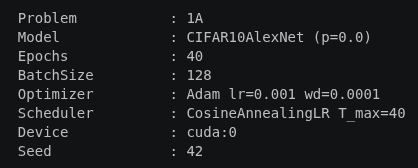
\includegraphics[width=\linewidth]{../../hw1/output/q1/hyperParams.png}
            \caption{\textbf{Hyper Parameters Used to Train the Model}}
            \label{fig:1a_hyperParams}
    \end{center}
\end{figure}

\begin{figure}[H]
    \begin{center}
            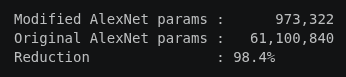
\includegraphics[width=\linewidth]{../../hw1/output/q1/1a_paramCount.png}
            \caption{\textbf{Total Countable Parameters between Original and Modified AlexNet}}
            \label{fig:1a_paramCount}
    \end{center}
\end{figure}

\begin{figure}[H]
    \begin{center}
            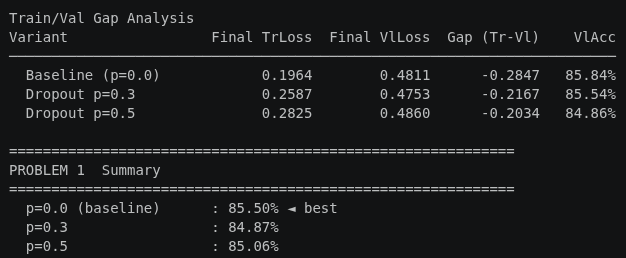
\includegraphics[width=\linewidth]{../../hw1/output/q1/1b_gap_analysies.png}
            \caption{\textbf{Training and Validation Gap Analysis}}
            \label{fig:1a_gapAnalysis}
    \end{center}
\end{figure}

\begin{figure}[H]
    \begin{center}
            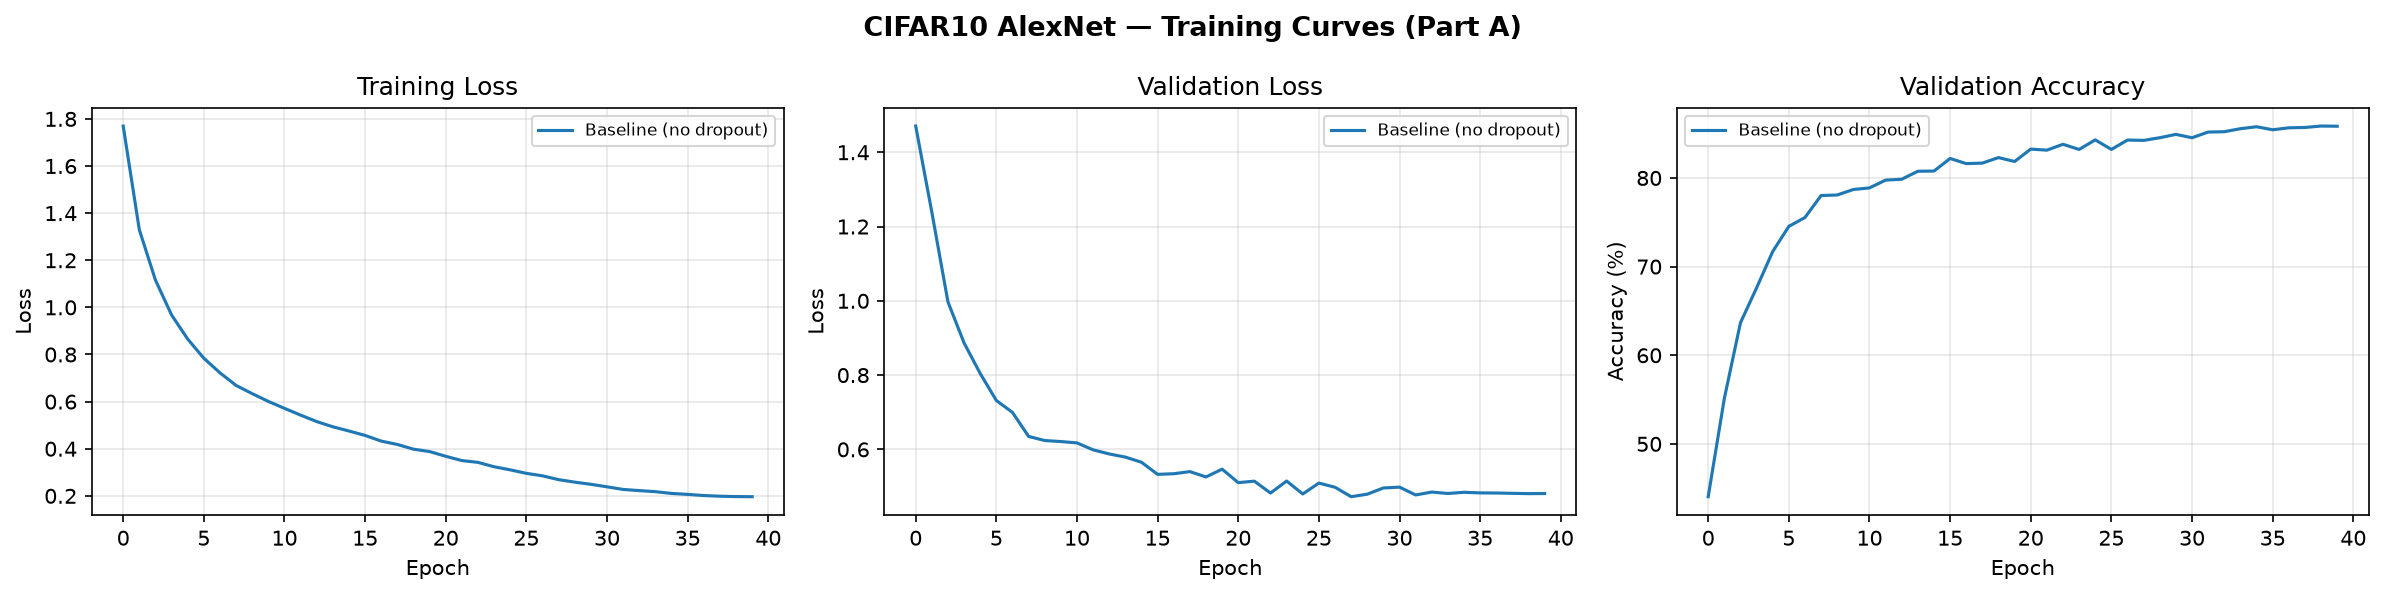
\includegraphics[width=\linewidth]{../../hw1/output/q1/1a_training_curves.png}
            \caption{\textbf{Training Curves for part A}}
            \label{fig:1a_trainingCurves}
    \end{center}
\end{figure}

\begin{figure}[H]
    \begin{center}
            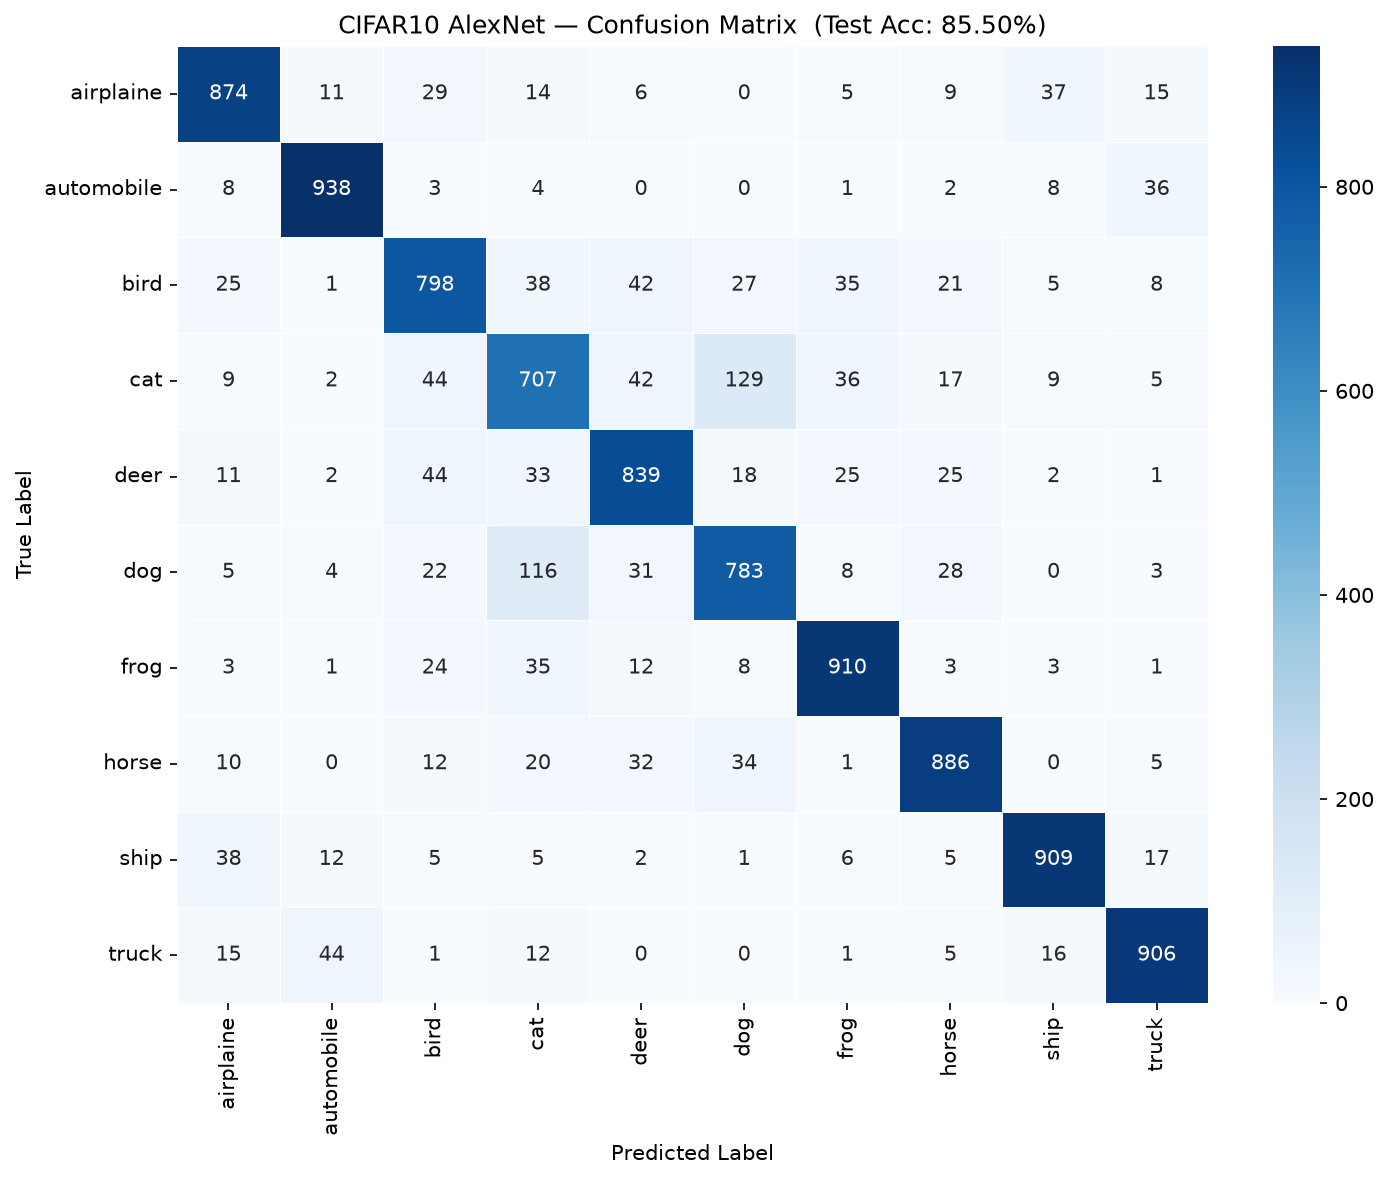
\includegraphics[width=\linewidth]{../../hw1/output/q1/1a_confusion_matrix.png}
            \caption{\textbf{Confusion Matrix for part A}}
            \label{fig:1a_confusionMatrix}
    \end{center}
\end{figure}

\begin{figure}[H]
    \begin{center}
            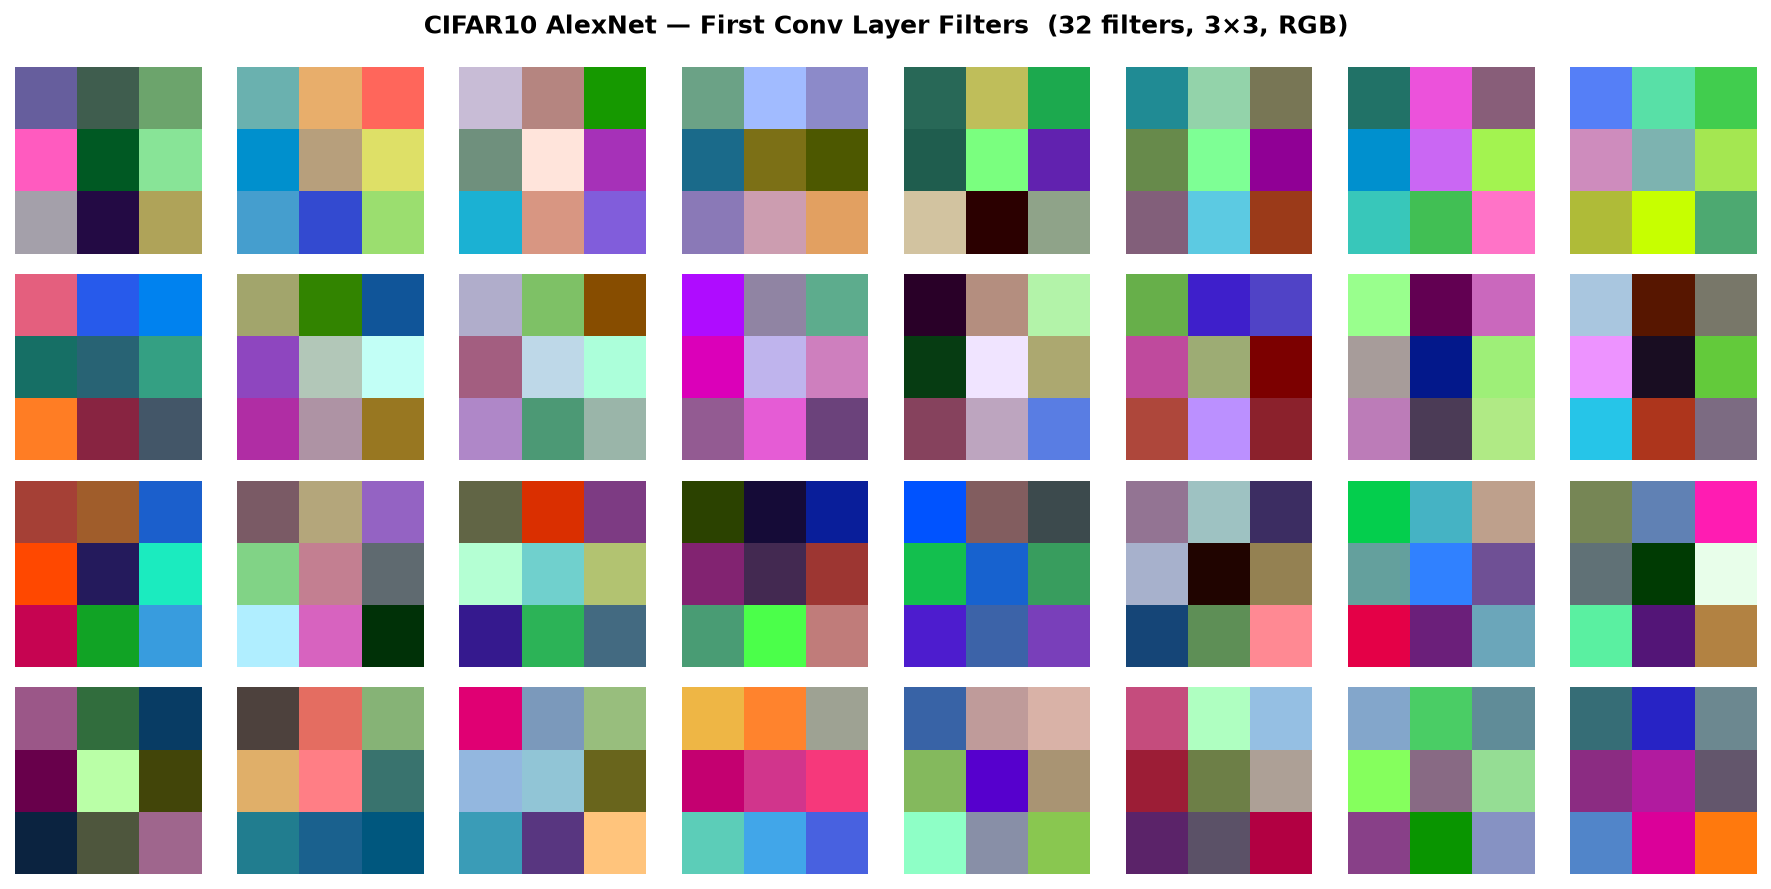
\includegraphics[width=\linewidth]{../../hw1/output/q1/1a_filters.png}
            \caption{\textbf{Filters for part A}}
            \label{fig:1a_filters}
    \end{center}
\end{figure}

\begin{figure}[H]
    \begin{center}
        \begin{subfigure}{0.5\linewidth}
            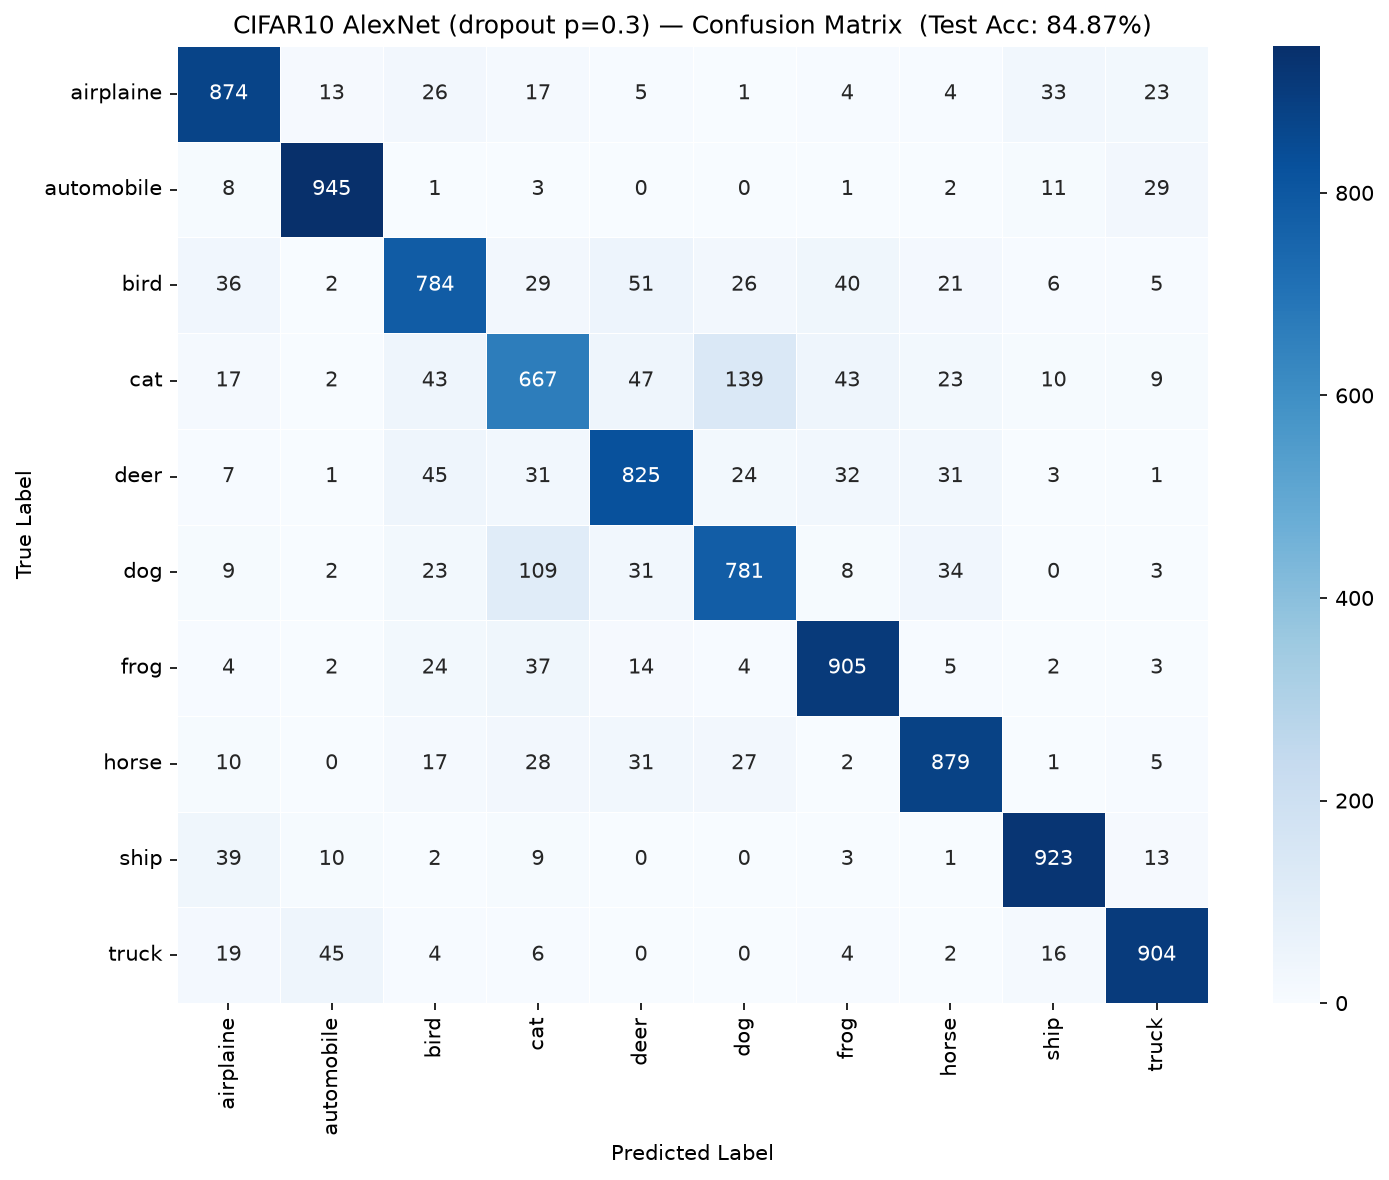
\includegraphics[width=\linewidth]{../../hw1/output/q1/1b_cm_p03.png}
            \caption{Drouput = 0.3}
            \label{fig:1b_p03CM}
        \end{subfigure}
        \hfill
        \begin{subfigure}{0.5\linewidth}
            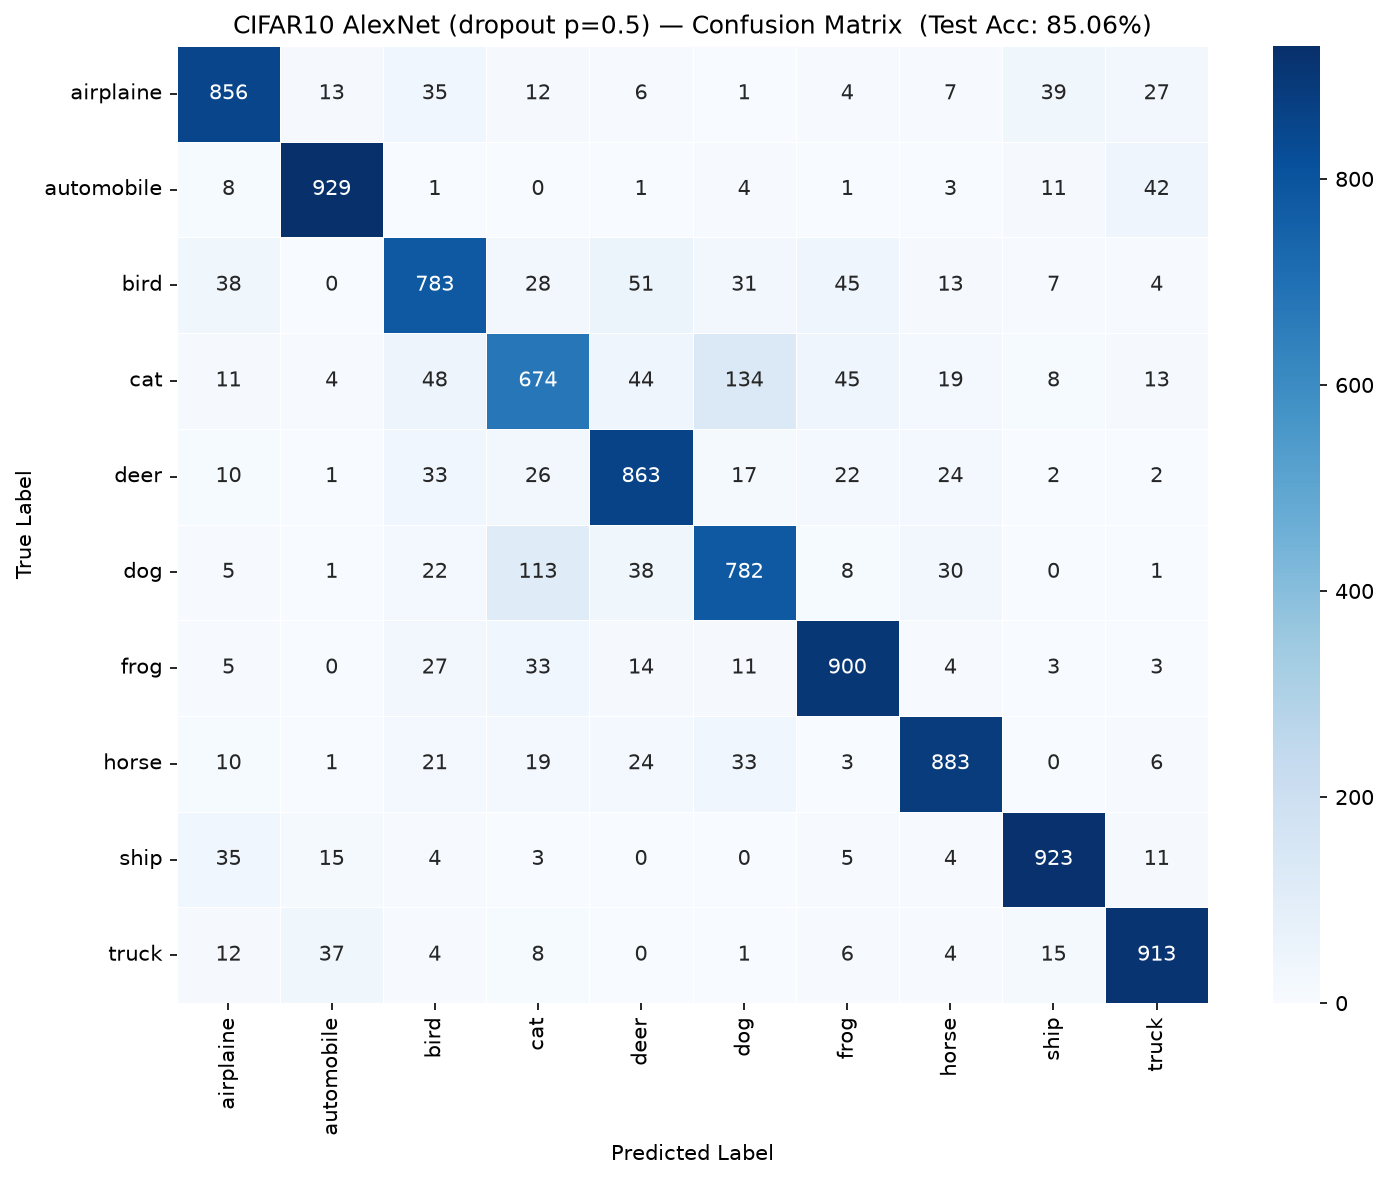
\includegraphics[width=\linewidth]{../../hw1/output/q1/1b_cm_p05.png}
            \caption{Drouput = 0.5}
            \label{fig:1b_p05}
        \end{subfigure}
        \caption{Confusion Matrices for Different Dropouts}
    \end{center}
\end{figure}

\begin{figure}[H]
    \begin{center}
            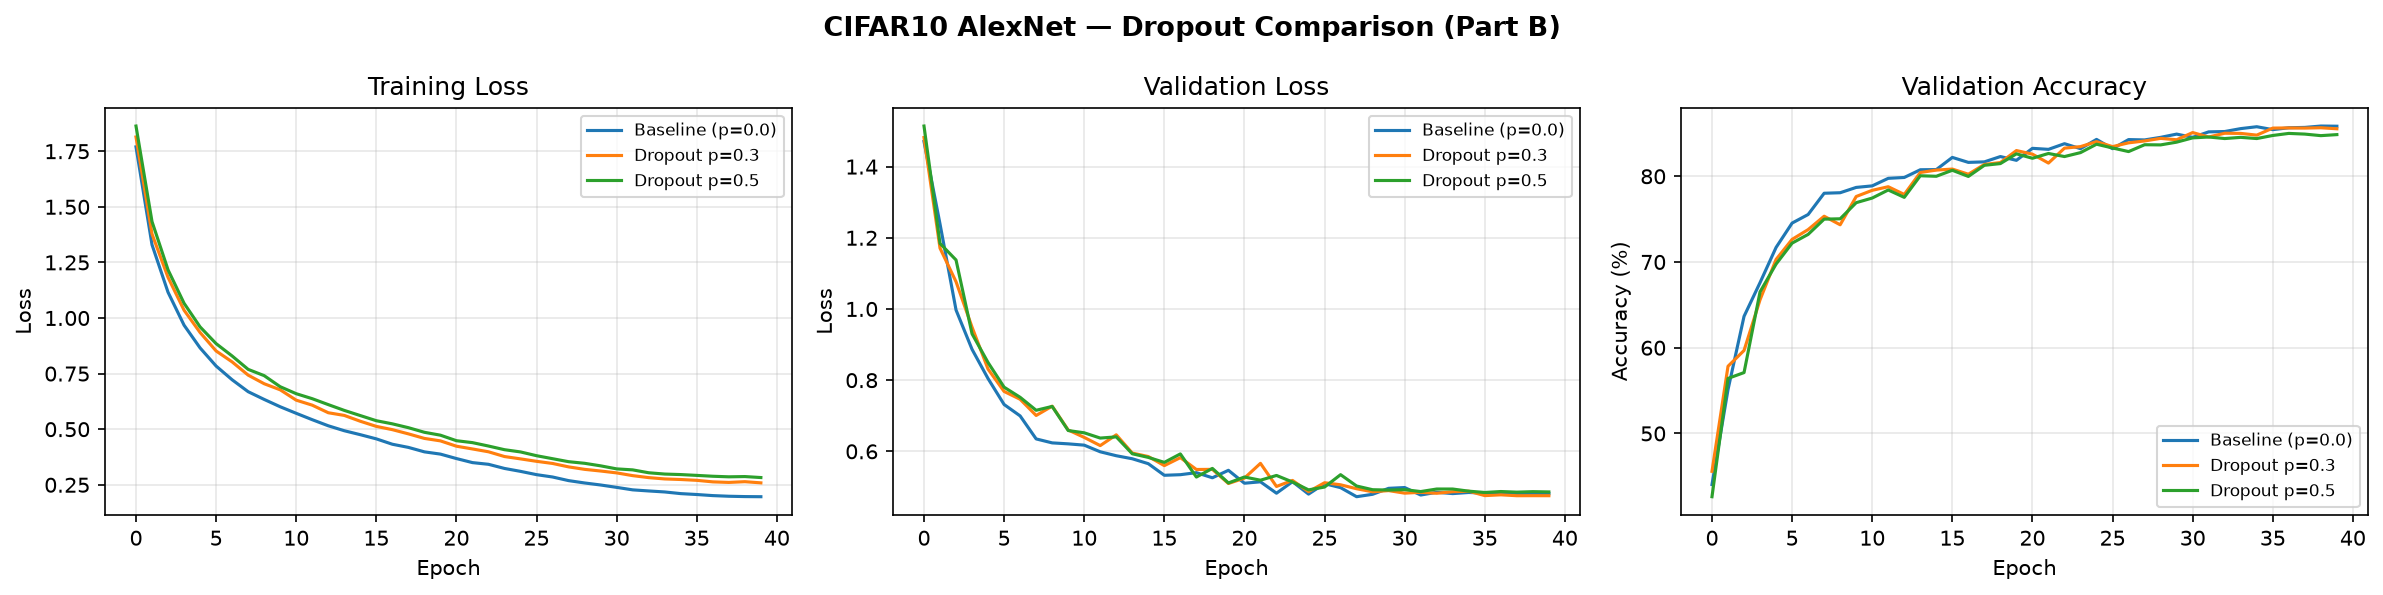
\includegraphics[width=\linewidth]{../../hw1/output/q1/1b_dropout_comparison.png}
            \caption{\textbf{Comparison between Dropouts}}
            \label{fig:1b_dropComp}
    \end{center}
\end{figure}

\section*{\textbf{Problem 2}}

\textbf{Objective} Pick a suitable VGG configuration (from 11 to 19) whose adapted parameter count is closest to the modified AlexNet, train it under the same conditions, and compare the two architectures.

With the increase in convolution layers stacked between each pool it becomes more difficult to constrain all the additional parameters with the fixed amount of data that CIFAR-10 provides. In addition, the additional layers provide a costly overhead and finer depth that is not required for the CIFAR-10 dataset.

\begin{table}[H]
    \centering
    \label{tab:vgg11xChanges}
    \caption{\textbf{Table Detailing all modficiations made to VGG-11}}
    \begin{tabular}{| c || c | c | c |}
        \hline 
        & \textbf{Component} & \textbf{Original VGG11} & \textbf{Modified VGG11} \\
        \hline
        \textbf{1.} & Filter Scale Factor & N/A & $\div 4$ \\
        \hline
        \textbf{2.} & Filter Cap & 512 & 128 \\
        \hline
        \textbf{3.} & Final Spatial Map & 7x7 & 1x1 \\
        \hline
        \textbf{4.} & Input to FC & 512x7x7 & 128x1x1 \\
        \hline
        \textbf{5.} & FC Progression & $25,088 \rightarrow 4096 \rightarrow 4096 \rightarrow 4096 \rightarrow 1,000$ & $128 \rightarrow 1024 \rightarrow 1024 \rightarrow 256 \rightarrow 10$ \\
        \hline
    \end{tabular}
\end{table}

The reason for all the changes listed above are detailed down below:
\begin{enumerate}
    \item Due to CIFAR-10 having a lower resolution, the filters can be scaled down to reduce overhead and train the model at a more suitable capacity.
    \item At the final two stages, the spatial map is already 2x2 and 1x1 respectively. A higher dimensional flatten would be an unnecessary addition to the overhead cost of training the model.
    \item Since there are 8 layers being used on a 32x32 input, the final spatial map, as a direct consequence, will become 1x1 instead of the 7x7 achieved from the ImageNet input.
    \item If a bigger input were to be given to the FC, then this layer would dominate and undermine the convolution backbone, due to this a smaller, more reasonable input is given to allow the classifer to combine features without either one being dwarfed.
    \item The FC progression was changed for three main reasons. The first being that it had to rebuilt around the 128 convolution layer input, second the number of parameters being entered is not as big as the original ImageNet dataset, and finally, CIFAR-10 only has ten classes while the original had a thousand.
\end{enumerate}

\begin{figure}[H]
    \begin{center}
            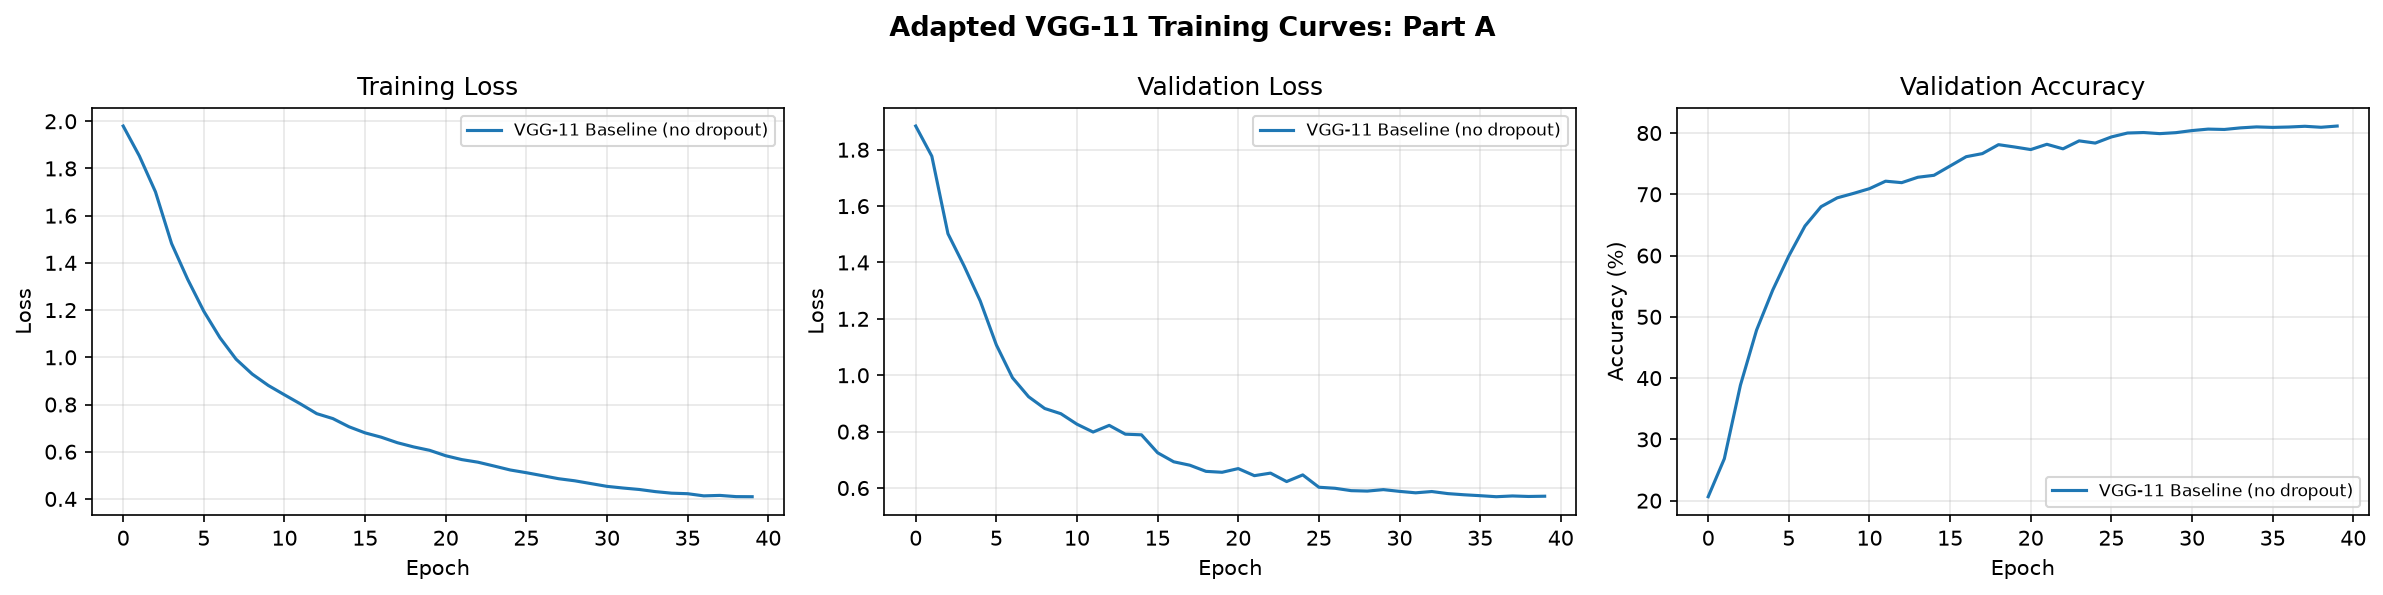
\includegraphics[width=\linewidth]{../../hw1/output/q2/2a_training_curves.png}
            \caption{\textbf{Training Curves for part A}}
            \label{fig:2a_trainingCurves}
    \end{center}
\end{figure}

\begin{figure}[H]
    \begin{center}
            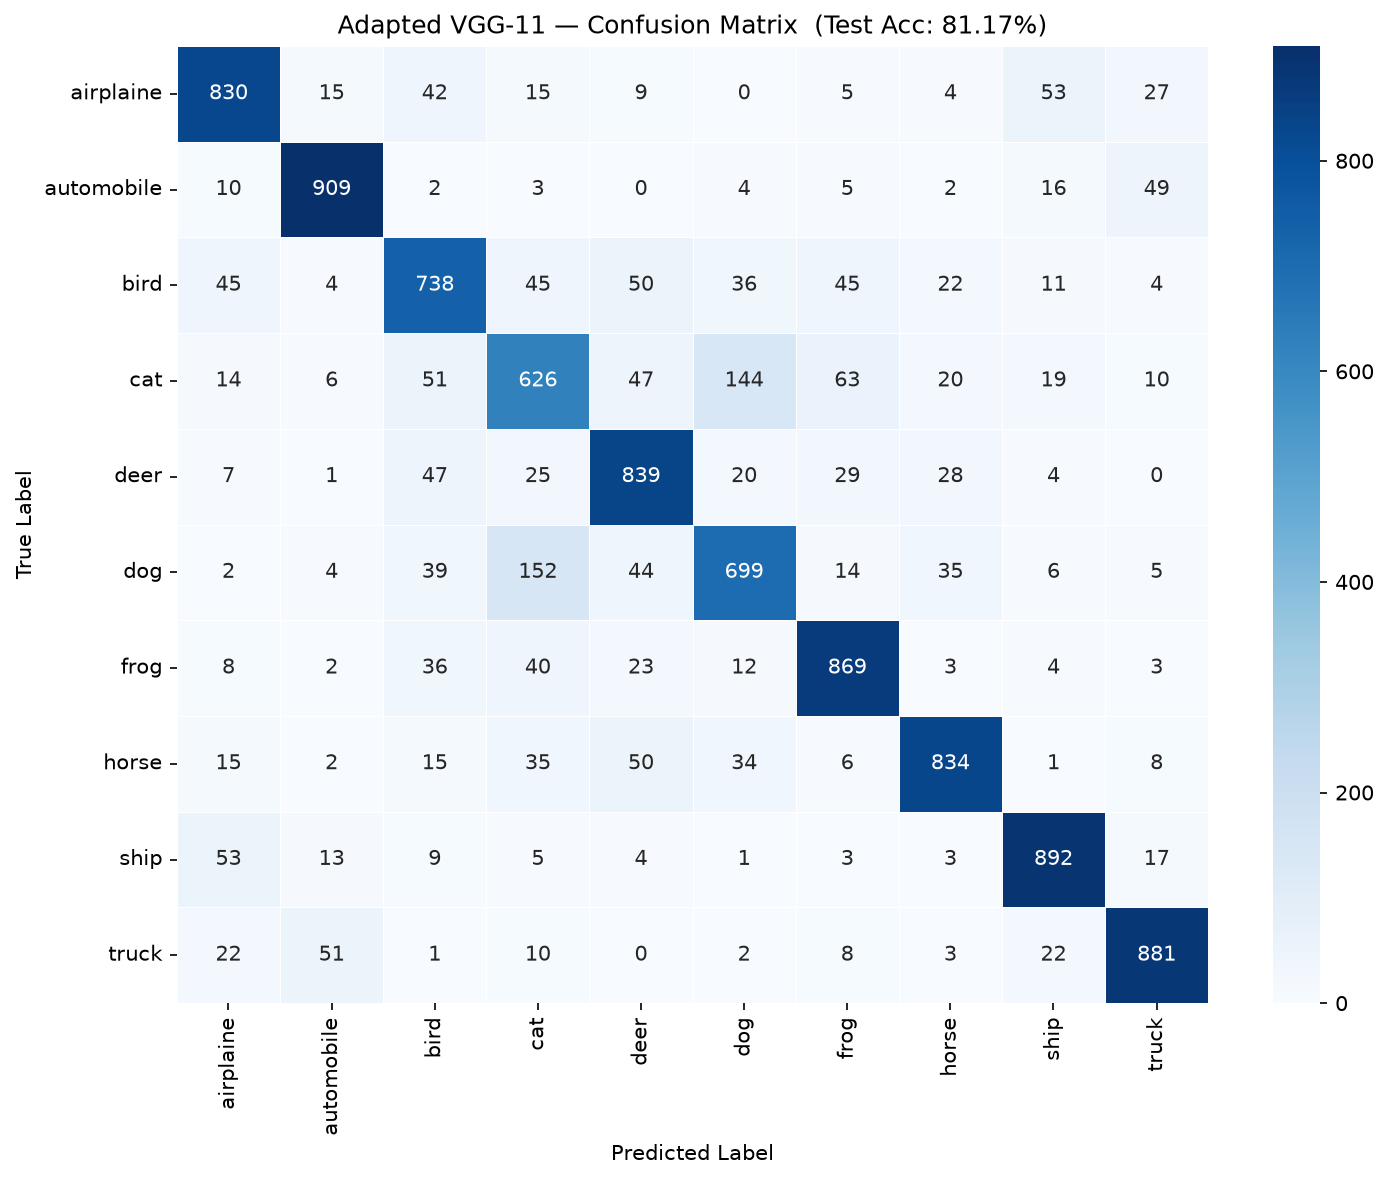
\includegraphics[width=\linewidth]{../../hw1/output/q2/2a_confusion_matrix.png}
            \caption{\textbf{Confusion Matrix for part A}}
            \label{fig:2a_confusionMatrix}
    \end{center}
\end{figure}

\begin{table}[H]
    \centering
    \label{tab:alexVGGComp}
    \caption{\textbf{Comparing Modified AlexNet and VGG11}}
    \begin{tabular}{| c || c | c | c |}
        \hline 
        & \textbf{Metric} & \textbf{Cifar-10 AlexNet} & \textbf{CIFAR-10 VGG11} \\
        \hline
        \textbf{1.} & Total Parameters & 973,322 & 974,186 \\
        \hline
        \textbf{2.} & Baseline Test Accuracy (\%) & 85.5 & 81.17 \\
        \hline
        \textbf{3.} & Best Test Accuracy (\%) & 85.5 & 81.26 \\
        \hline
        \textbf{4.} & Avg Epoch Training Time (s) & 3.7 & 3.65 \\
        \hline
        \textbf{5.} & Convergence Speed (No. of epochs) & N/A & 8 \\
        \hline
    \end{tabular}
\end{table}

Since AlexNet only have 5 convolution layers compared to VGG11's 8, it would definitely train faster per epoch along with the difference in the number of sequential layer operations need to be done. Similarly, the increased number of layers allows VGG-11 to generalise better as it is able to build abstract more features and with the former's unform 3x3 kernel design it is able to construct a more consistent feature hierarchy. The structural changes between both architectures that lead to their gap in accuracy and loss are depth, rate of spatial compression, reconstruction and class-score compression, and finally dropout interaction.

\begin{figure}[H]
    \begin{center}
        \begin{subfigure}{0.5\linewidth}
            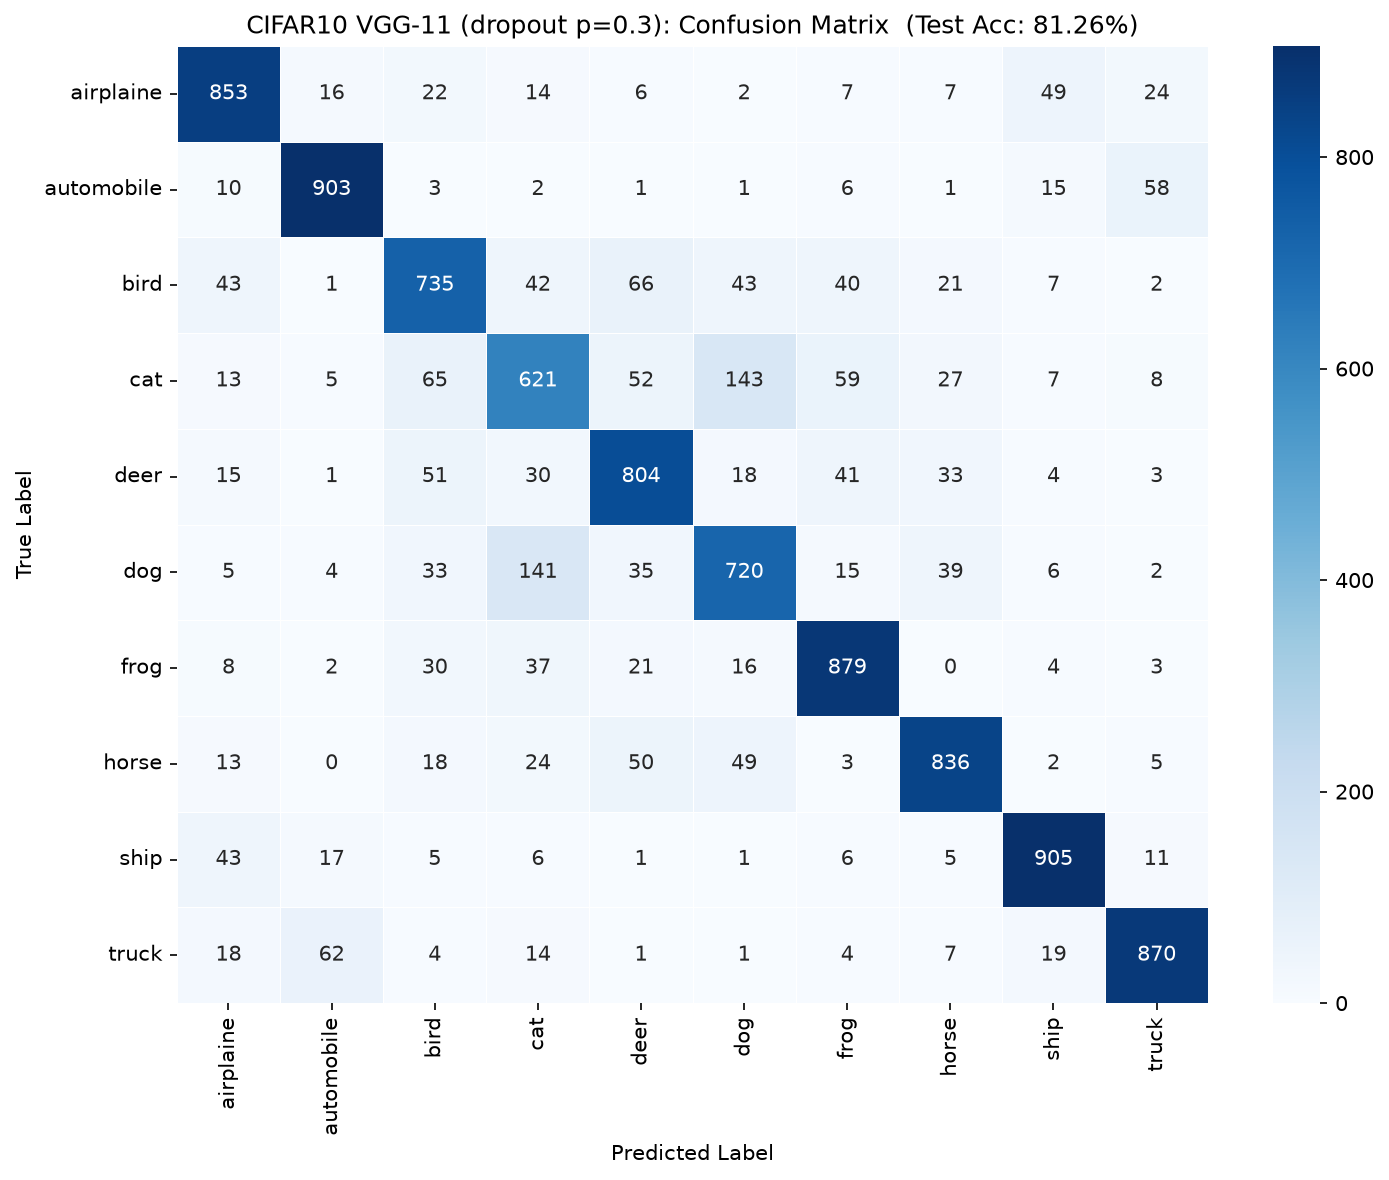
\includegraphics[width=\linewidth]{../../hw1/output/q2/2b_cm_p03.png}
            \caption{Drouput = 0.3}
            \label{fig:2b_p03CM}
        \end{subfigure}
        \hfill
        \begin{subfigure}{0.5\linewidth}
            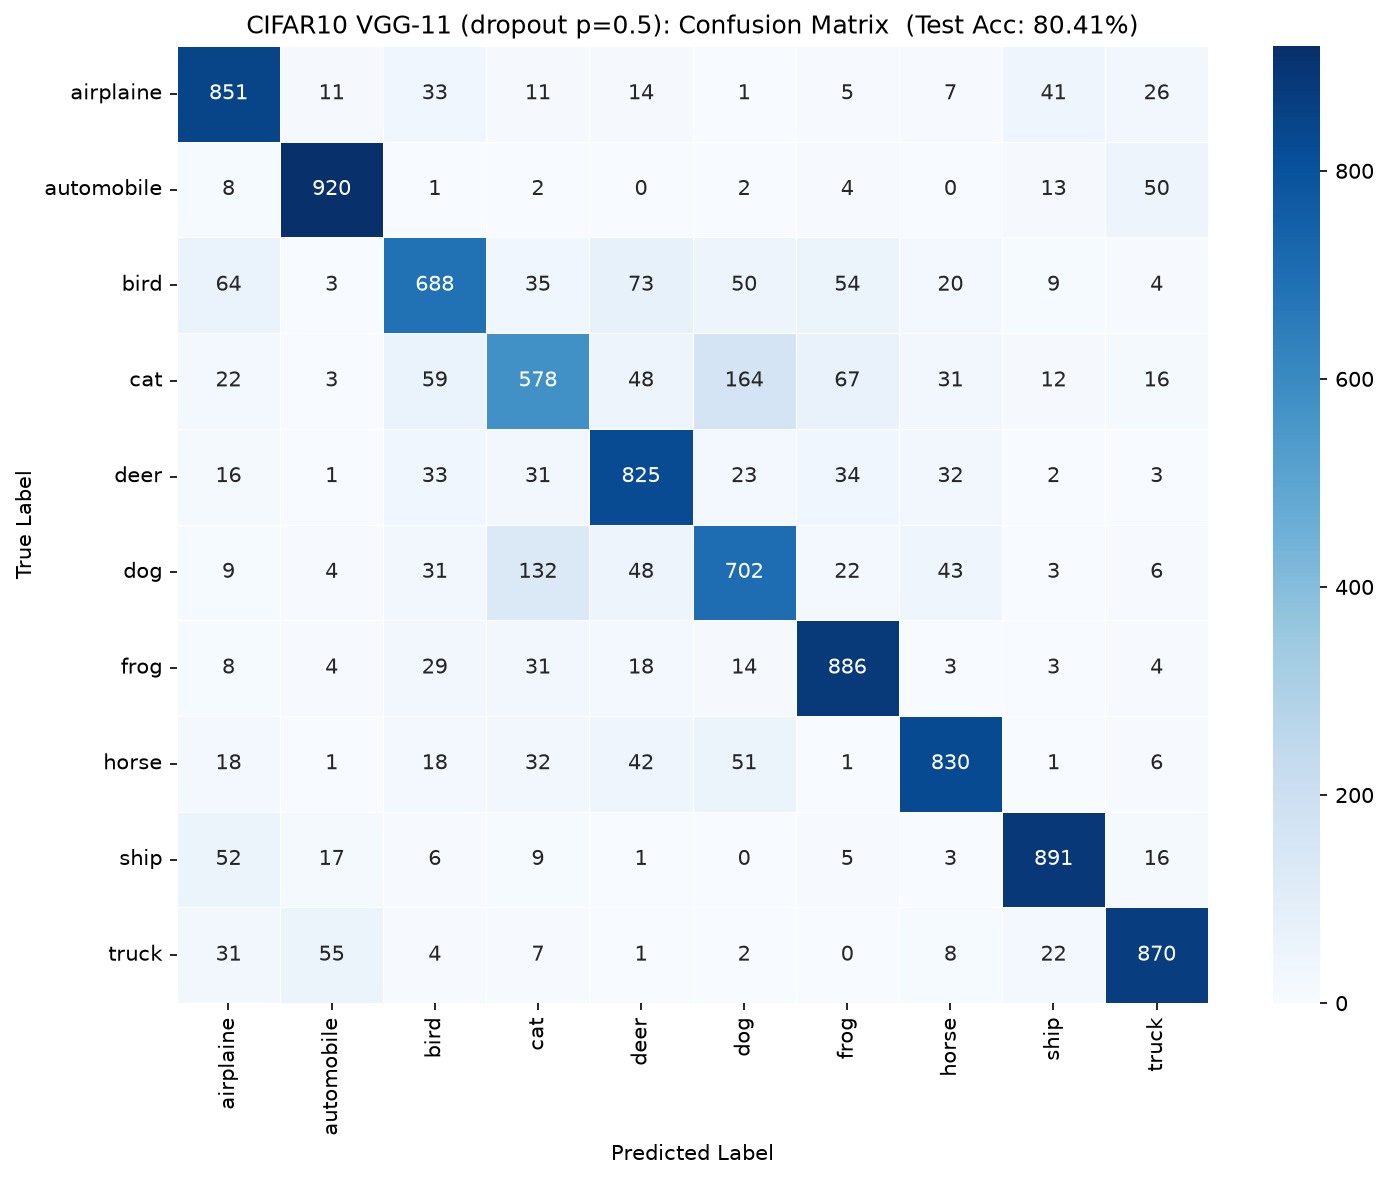
\includegraphics[width=\linewidth]{../../hw1/output/q2/2b_cm_p05.png}
            \caption{Drouput = 0.5}
            \label{fig:2b_p05}
        \end{subfigure}
        \caption{Confusion Matrices for Different Dropouts}
    \end{center}
\end{figure}

\begin{figure}[H]
    \begin{center}
            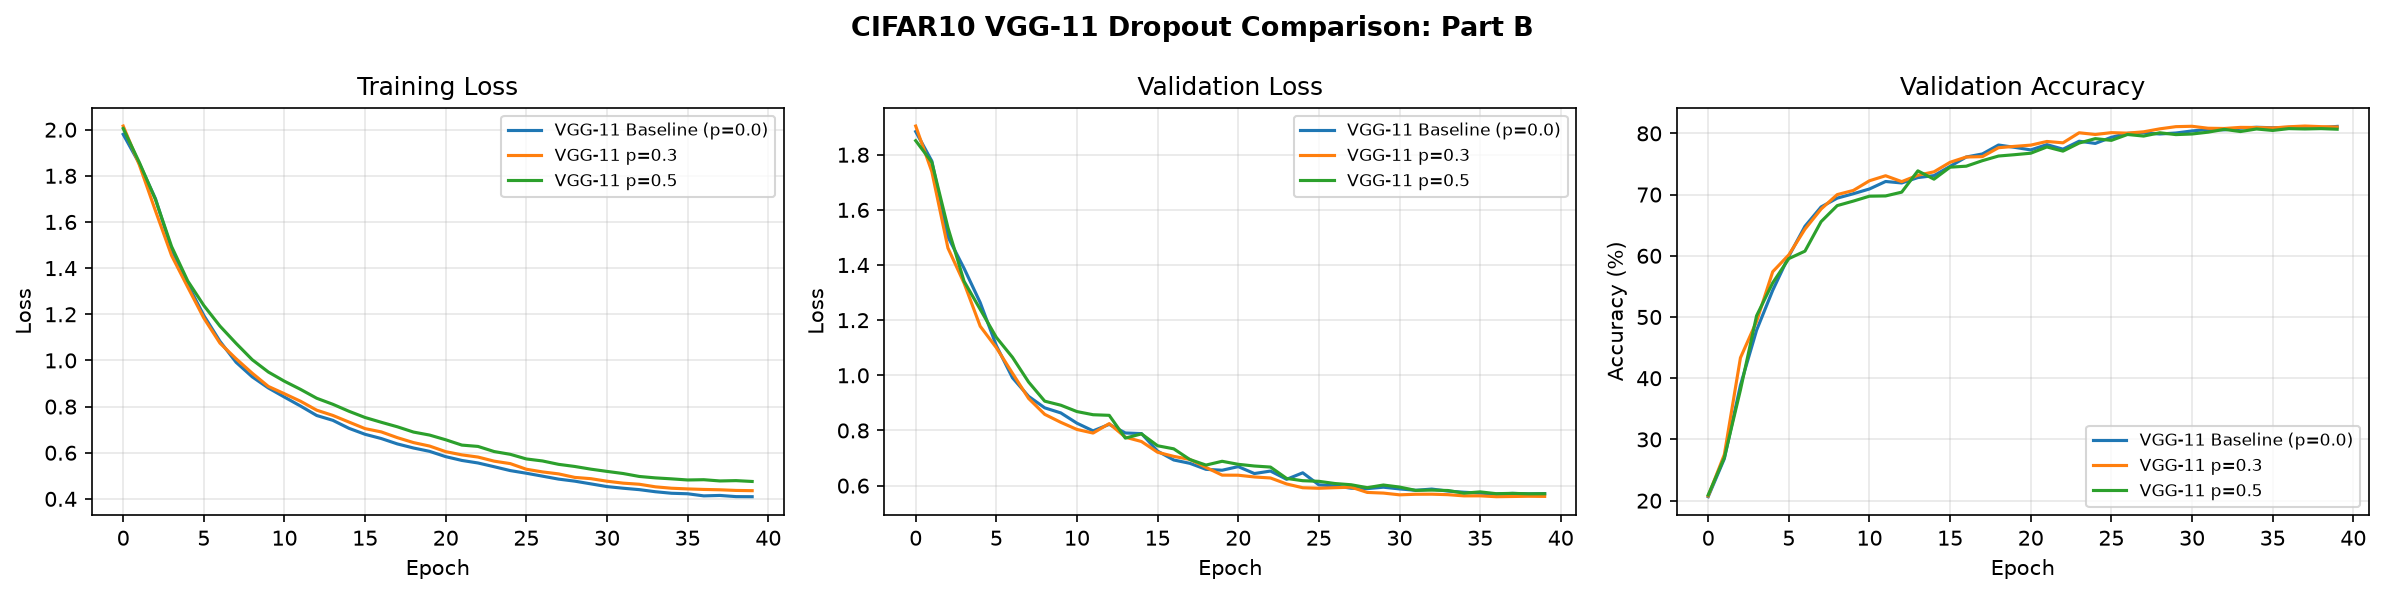
\includegraphics[width=\linewidth]{../../hw1/output/q2/2b_dropout_comparison.png}
            \caption{\textbf{Comparison between Dropouts}}
            \label{fig:2b_dropComp}
    \end{center}
\end{figure}

\begin{figure}[H]
    \begin{center}
            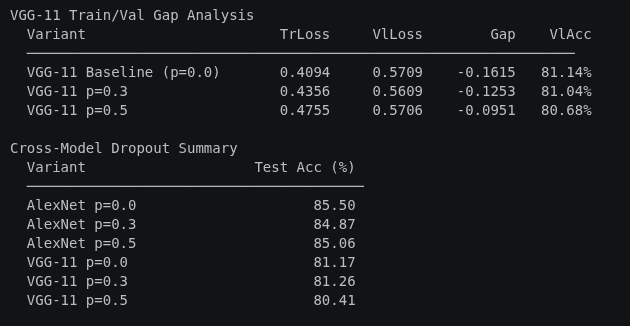
\includegraphics[width=\linewidth]{../../hw1/output/q2/crossModelDropout.png}
            \caption{\textbf{Comparison between Cross-Model Dropouts}}
            \label{fig:2b_modelDropComp}
    \end{center}
\end{figure}

A deeper architecture doesn't respond differently to dropout as the this only affects the FC layer whereas the depth is derived from the convolution layer backbone. However, due to the amount of information retained in VGG-11, the dropout does hurt slightly less compares to AlexNet.

\begin{table}[H]
    \centering
    \label{tab:bestVariantCrossModel}
    \caption{\textbf{Comparing Best Variant Performance}}
    \begin{tabular}{| c || c | c | c |}
        \hline 
        \textbf{Model} & \textbf{Baseline Acc (\%)} & \textbf{p=0.3 Acc (\%)}  & \textbf{p=0.5 Acc (\%)}\\
        \hline
        \textbf{CIFAR-10 AlexNet} & 85.5 (\textbf{BEST}) & 84.87 & 85.06 \\
        \hline
        \textbf{CIFAR-10 VGG-11} & 81.17 & 81.26 (\textbf{BEST}) & 80.41 \\
        \hline
    \end{tabular}
\end{table}

ALexNet outperformed VGG-11 as seen in the table above. A possible reason for this could be the fact that VGG-11 over-pooled the spatial map constricting it to 128x1x1 which then needs to be expanded in the FC layers whereas AlexNet does not. This could result in some loss of information.

\section*{\textbf{Problem 3}}

\textbf{Objective:} Implement ResNet-18 from scratch, compare it against ResNet-11, and study how added depth affects performance and regularization.

Both ResNet-11 and 18 share the same general architecture details, these being:
\begin{enumerate}
    \item The main path, as specified in the problem is, 3x3 conv, BN, ReLU, 3x3 conv, BN, skip connection.
    \item They share the same skip path.
    \item They both output as ReLU(main-path(x) + skip-path(x))
    \item No bias due to batch normalization
    \item As seen above, after every convolution layer both models go through batch normalization.
\end{enumerate}

The difference in architecture arises in the number of BasicBlocks that both have for each of their 4 stages. ResNet-11 has 1 BasicBlock for all 4 stages with 64, 128, 256, and 512 channels respectively in addition to a stride of 2 for every stage except the first, which has a stride of 1. ResNet-18 follows along in regards to channels and strides but has 2 BasicBlocks per stage.
Moving on, these 2 models have introduced skip connections. Skip connections are the solution applied in deep neural networks to combat against the problem of the vanishing gradient. To prevent the shrinkage of the gradient during back propogation, a skip connection bypasses the 2 convolution layers completely and adds the input to the output. During the forward pass this helps get rid of learning anything unnecessary, sometimes only learning what to add to the input and sometimes learning nothing. Skip connections shine during the back passes when the gradient becomes so small, that the skip connection is always there to add something meaningful regardless of depth. There are 2 skip connections used in this problem. When the input and output are of the same spatial size and channel count, the input is directly added. When channels or stride increases the input is trasnformedto match the dimensions of the output and then added. For models like ResNet-11 and 18 that have 9 and 17 convolution layers respectively, these skip connections are crucial to ensure proper training of the models.

\begin{figure}[H]
    \begin{center}
        \begin{subfigure}{\linewidth}
            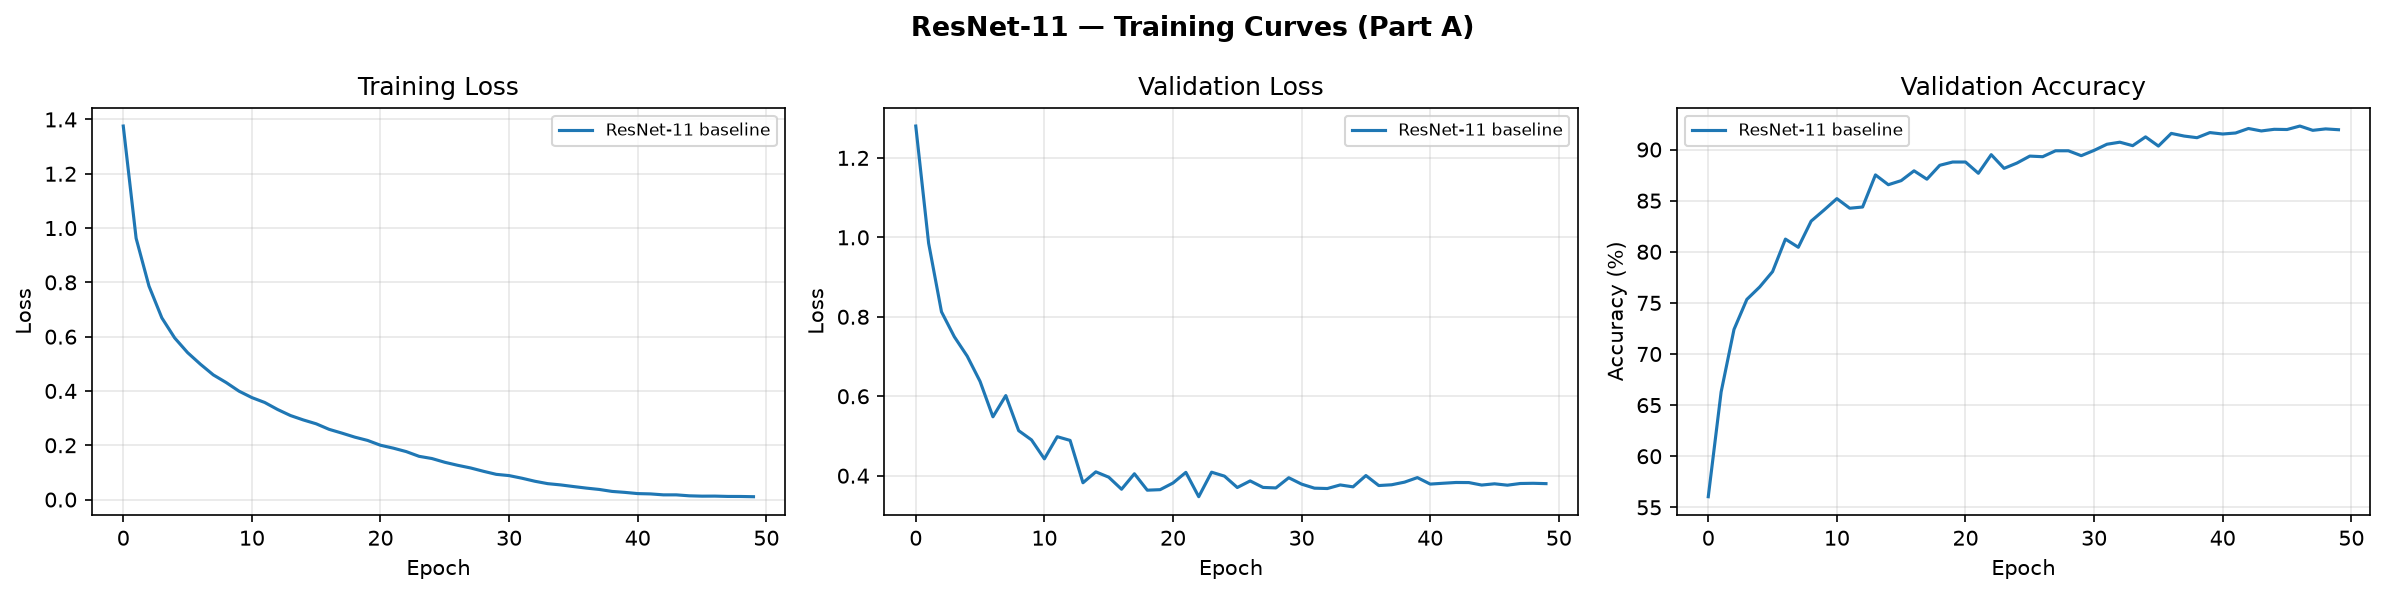
\includegraphics[width=\linewidth]{../../hw1/output/q3/3a_r11_curves.png}
            \caption{\textbf{ResNet-11}}
            \label{fig:3a_r11Curve}
        \end{subfigure}
        \hfill
        \begin{subfigure}{\linewidth}
            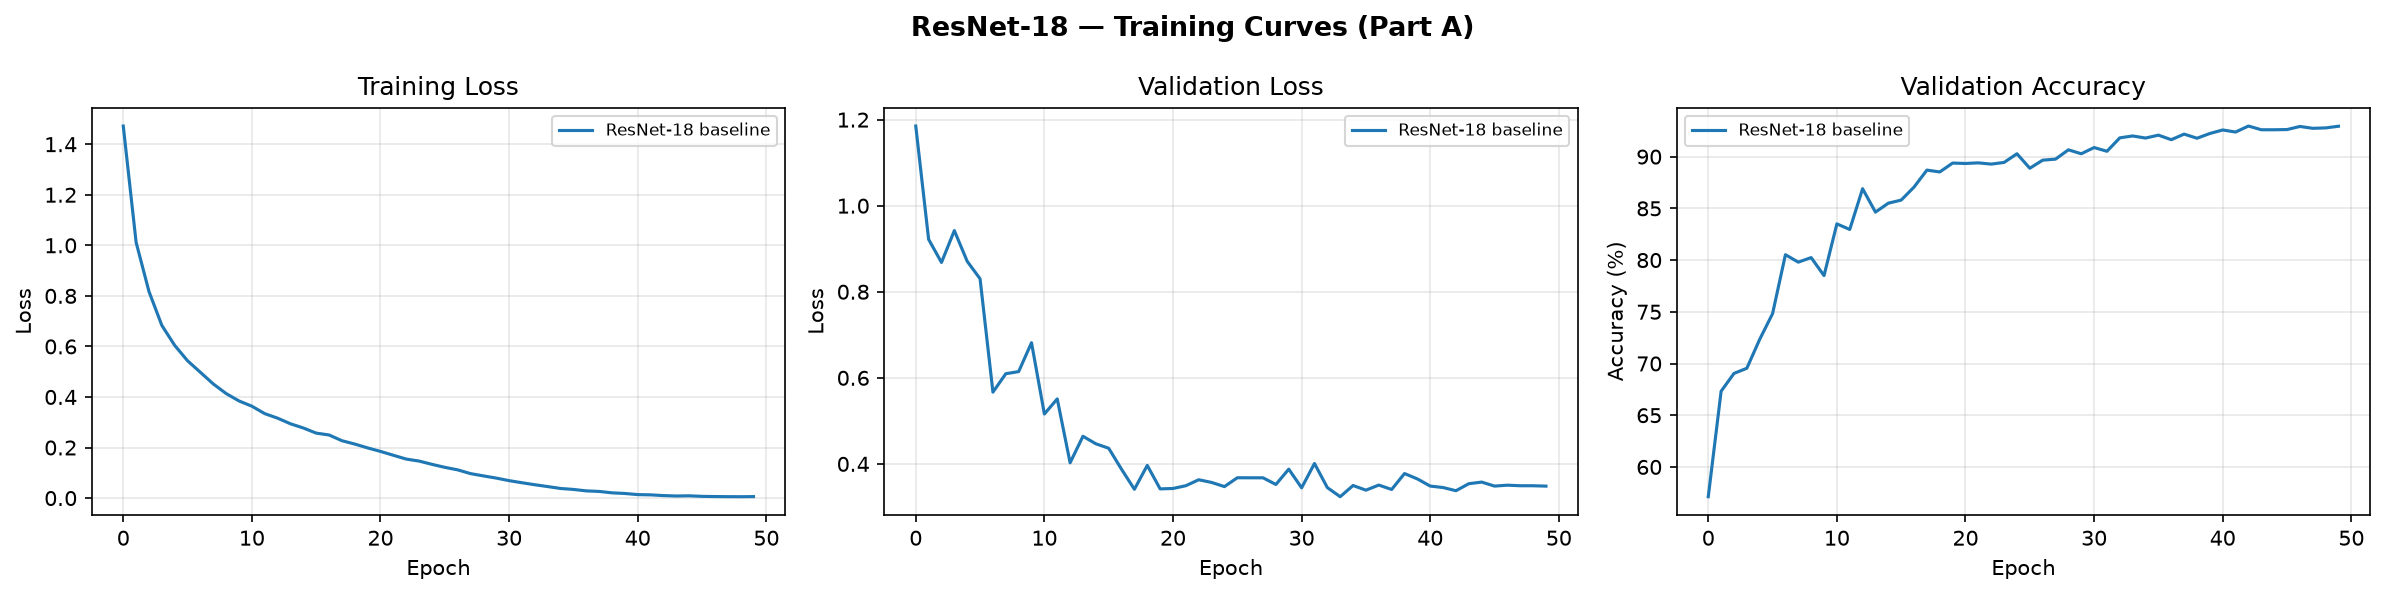
\includegraphics[width=\linewidth]{../../hw1/output/q3/3a_r18_curves.png}
            \caption{\textbf{ResNet-18}}
            \label{fig:3a_r18Curves}
        \end{subfigure}
        \caption{\textbf{Training Curves for Part A for both models}}
    \end{center}
\end{figure}

\begin{figure}[H]
    \begin{center}
        \begin{subfigure}{\linewidth}
            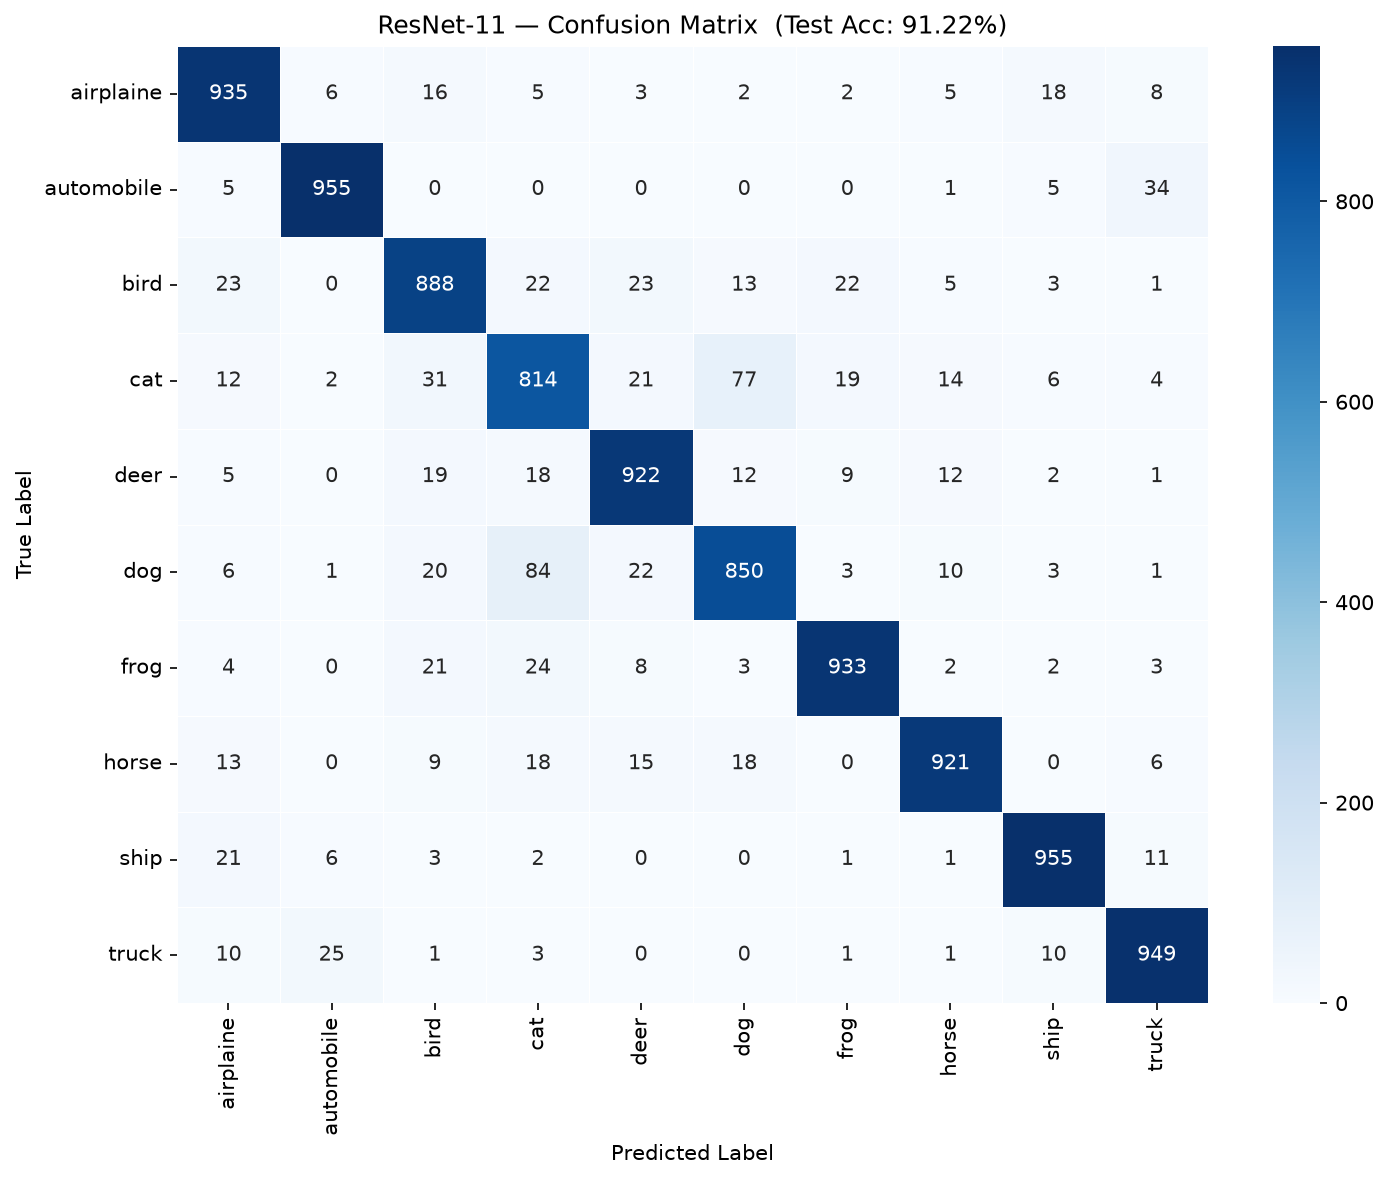
\includegraphics[width=\linewidth]{../../hw1/output/q3/p3a_r11_cm.png}
            \caption{\textbf{ResNet-11}}
            \label{fig:3a_r11Conf}
        \end{subfigure}
        \hfill
        \begin{subfigure}{\linewidth}
            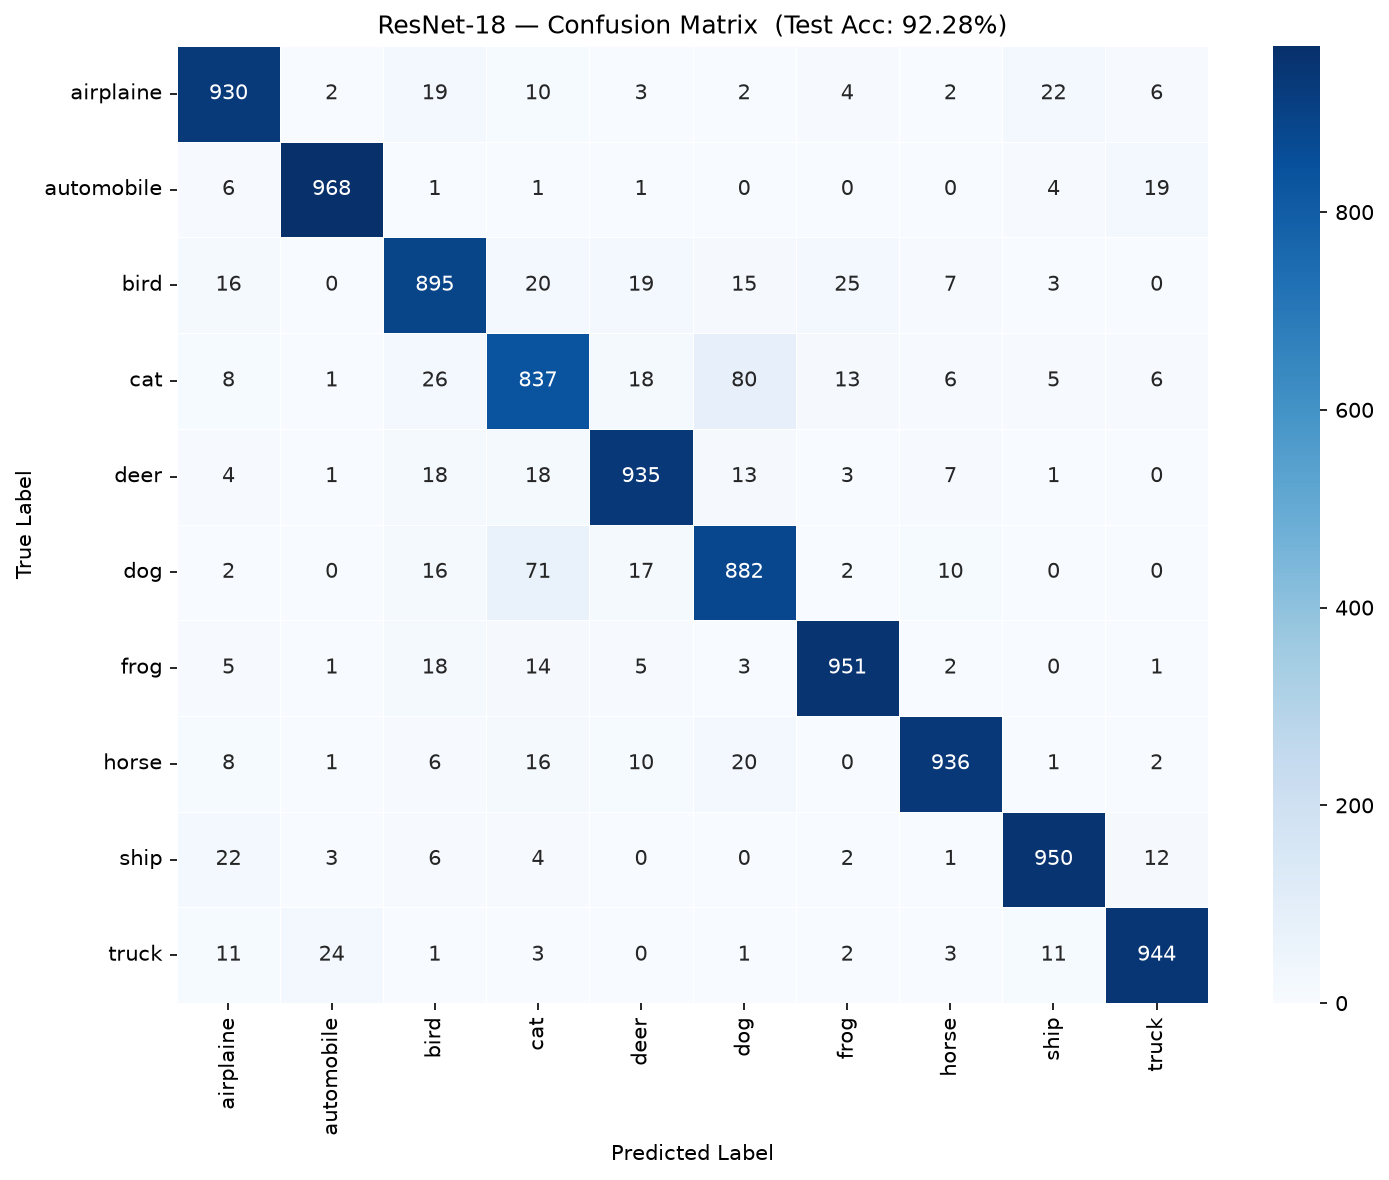
\includegraphics[width=\linewidth]{../../hw1/output/q3/p3a_r18_cm.png}
            \caption{\textbf{ResNet-18}}
            \label{fig:3a_r18Conf}
        \end{subfigure}
        \caption{\textbf{Training Curves for Part A for both models}}
    \end{center}
\end{figure}

\begin{figure}[H]
    \begin{center}
            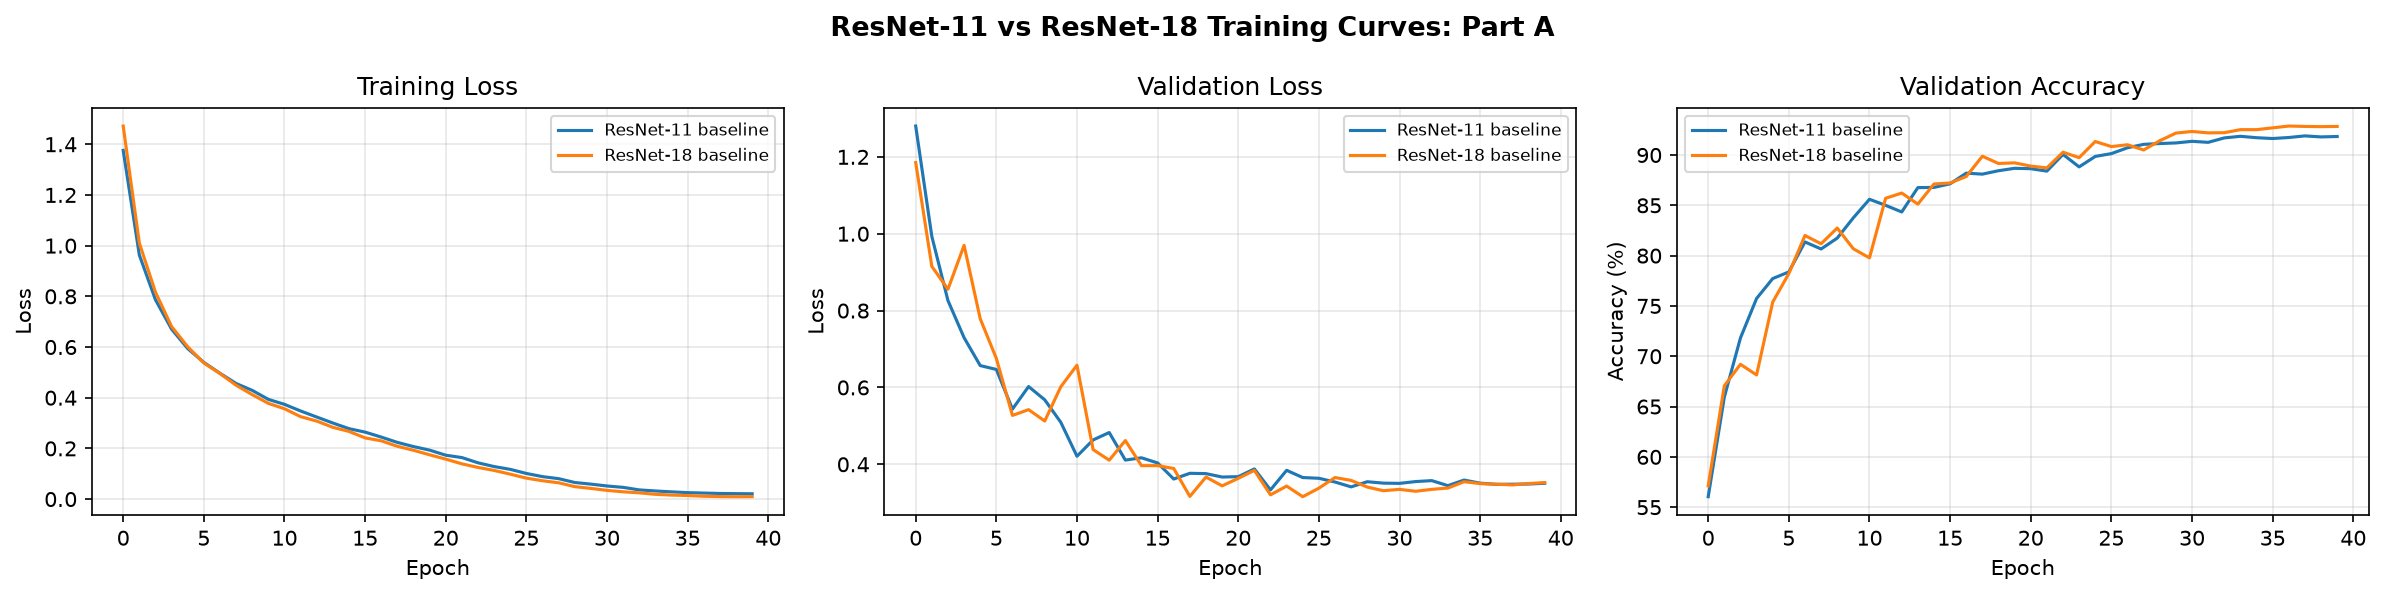
\includegraphics[width=\linewidth]{../../hw1/output/q3/3a_resnet_comparison.png}
            \caption{\textbf{Comparison between ResNet Models}}
            \label{fig:3a_rModelComp}
    \end{center}
\end{figure}

Due to the low resolutions of the CIFAR-10 dataset, the added depth provided by ResNet-18 is not worth the cost as this is a very over-engineered solution for such broad categories that do not require all the extra information that is being provided by this model. Therefore, I believe the added depth is not wortht the cost.

\begin{figure}[H]
    \begin{center}
        \begin{subfigure}{\linewidth}
            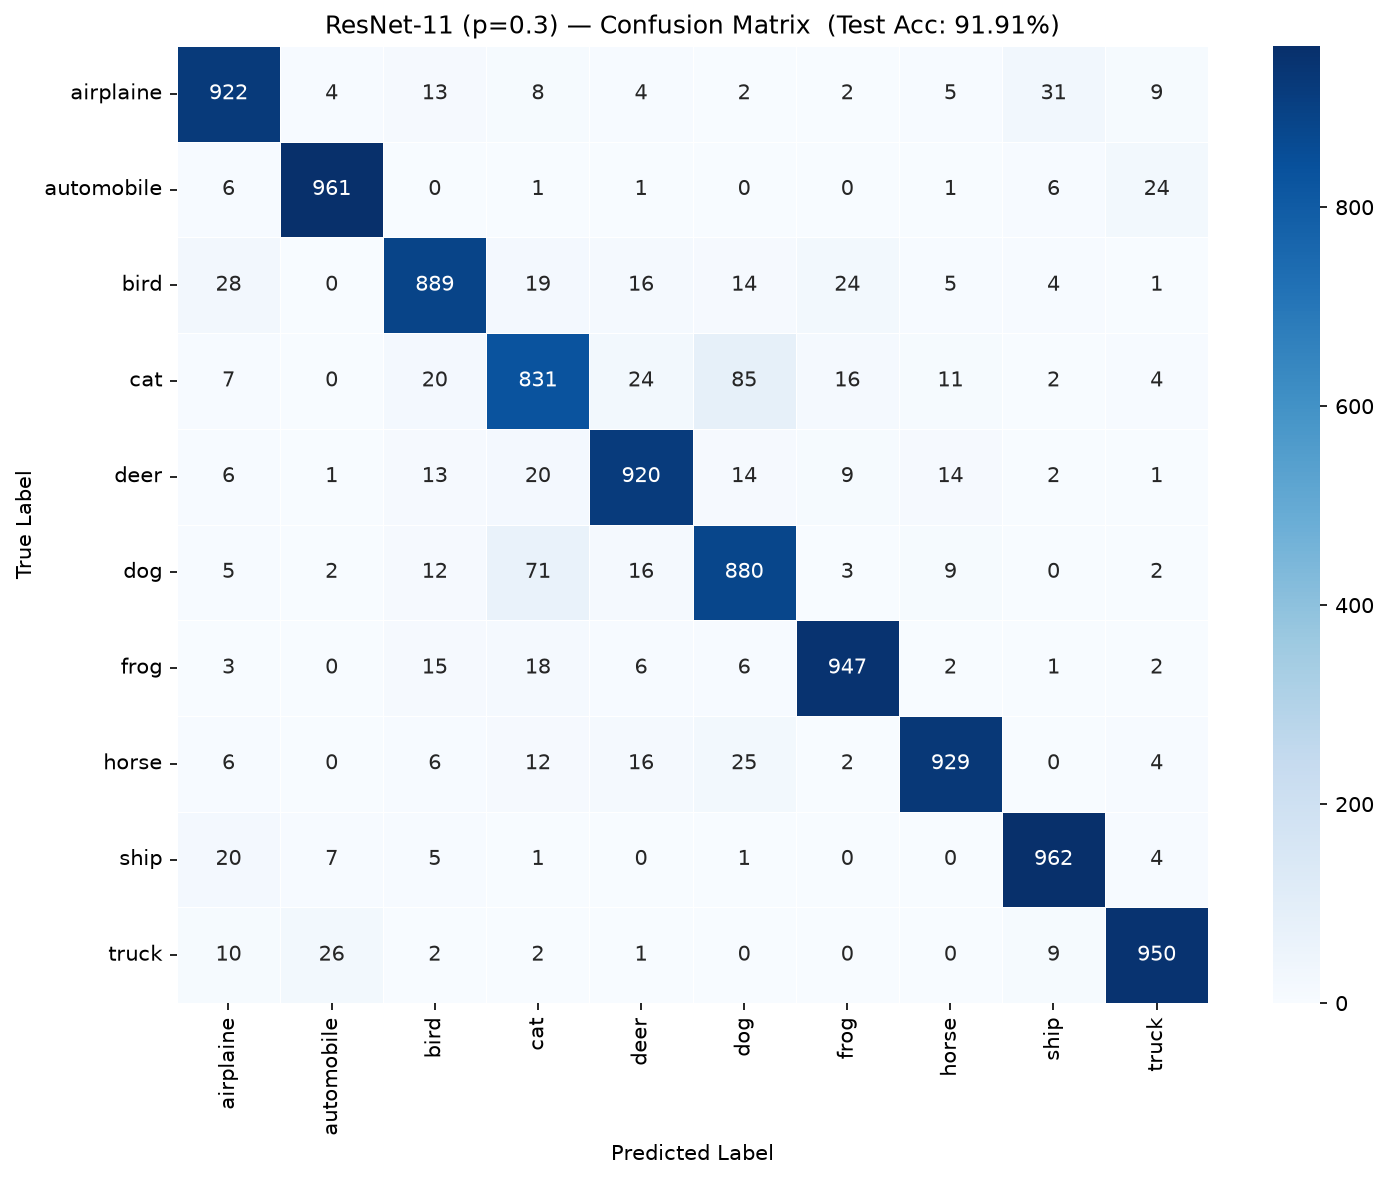
\includegraphics[width=\linewidth]{../../hw1/output/q3/3b_r11_cm_p03.png}
            \caption{Drouput = 0.3}
            \label{fig:3b_r11p03CM}
        \end{subfigure}
        \hfill
        \begin{subfigure}{\linewidth}
            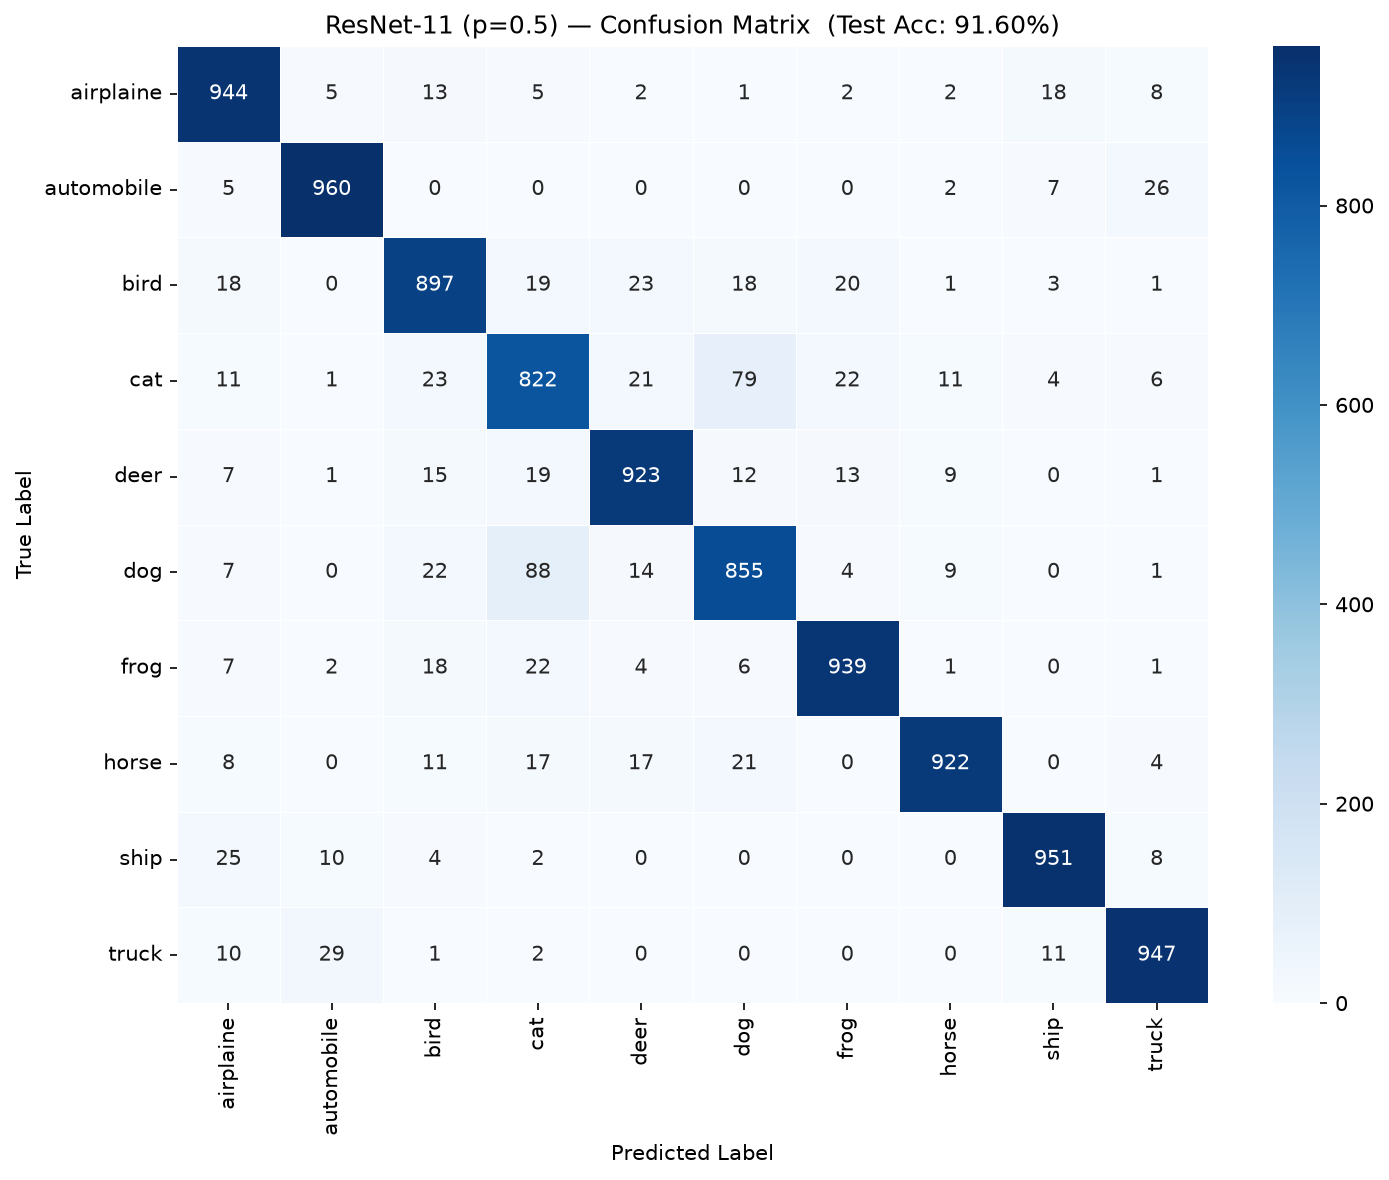
\includegraphics[width=\linewidth]{../../hw1/output/q3/3b_r11_cm_p05.png}
            \caption{Drouput = 0.5}
            \label{fig:3b_r11p05}
        \end{subfigure}
        \caption{Confusion Matrices for Different Dropouts for ResNet-11}
    \end{center}
\end{figure}

\begin{figure}[H]
    \begin{center}
        \begin{subfigure}{\linewidth}
            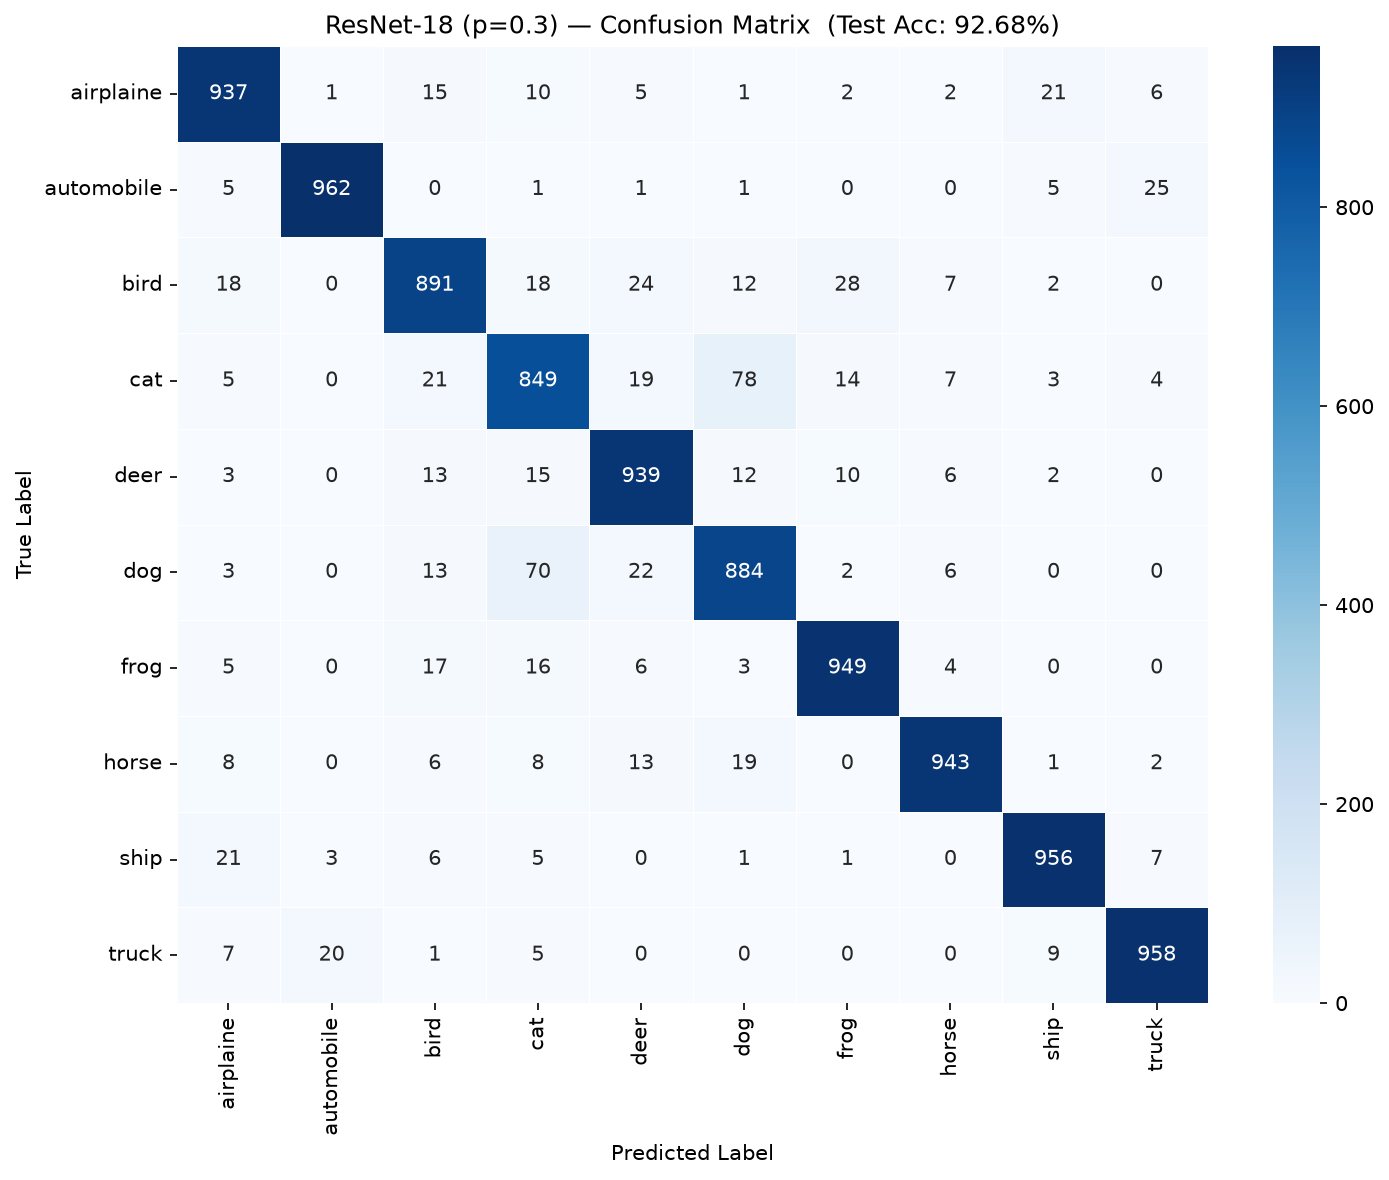
\includegraphics[width=\linewidth]{../../hw1/output/q3/3b_r18_cm_p03.png}
            \caption{Drouput = 0.3}
            \label{fig:3b_r18p03CM}
        \end{subfigure}
        \hfill
        \begin{subfigure}{\linewidth}
            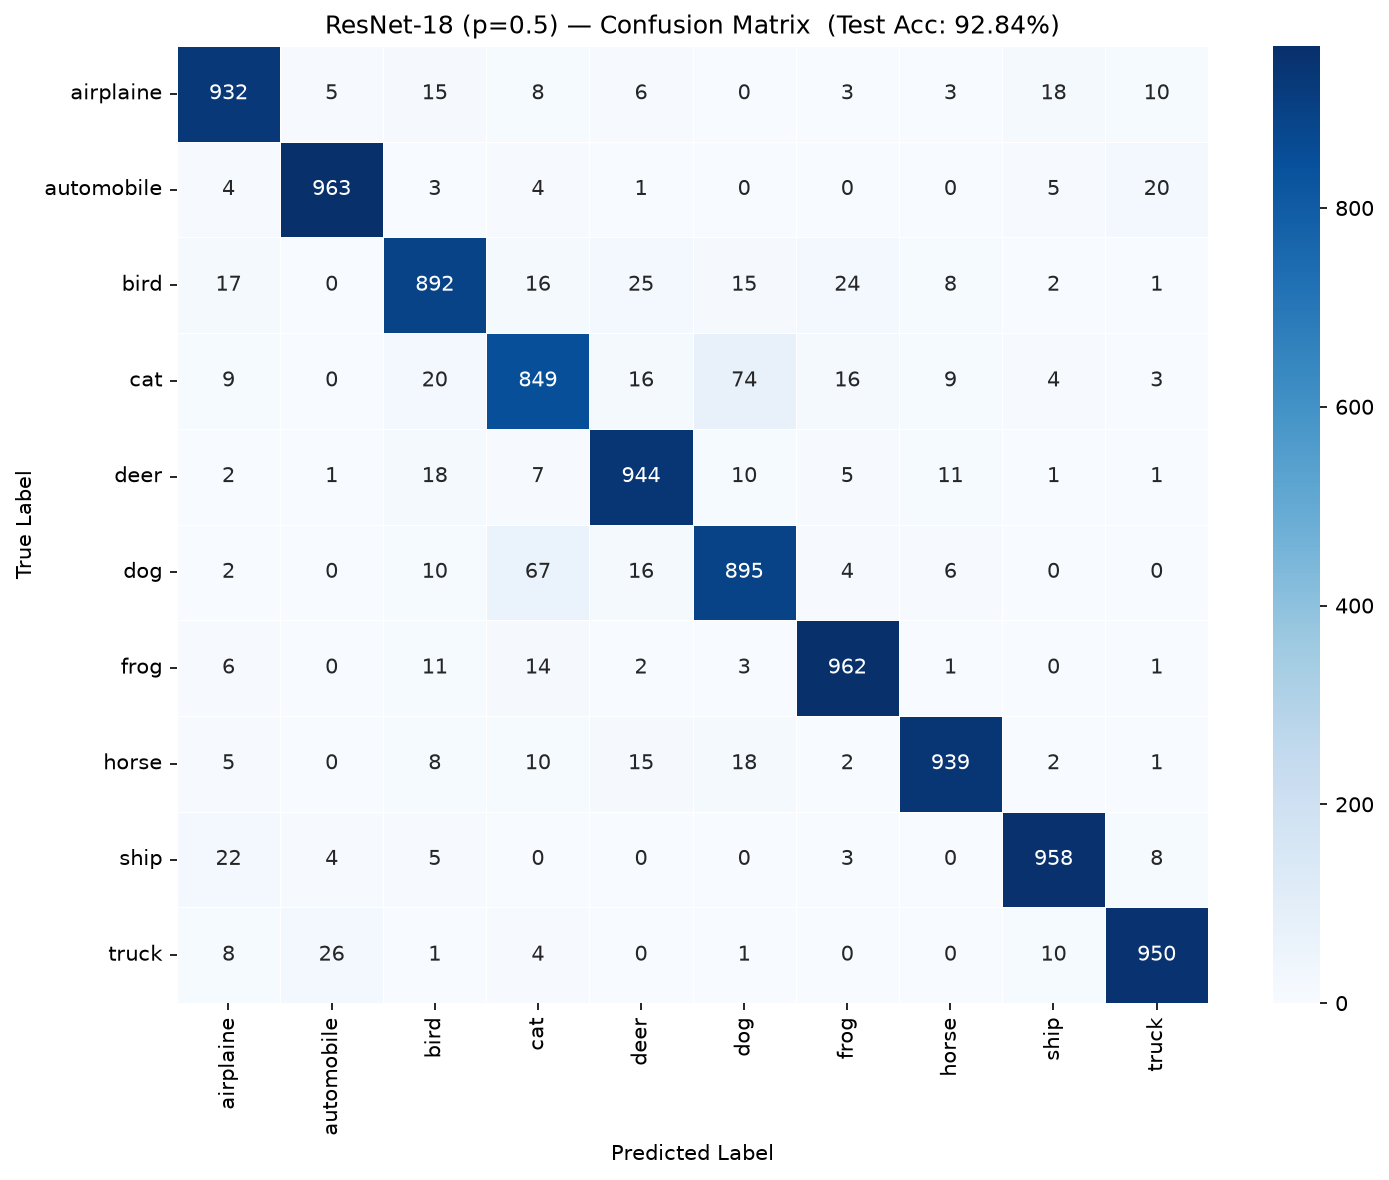
\includegraphics[width=\linewidth]{../../hw1/output/q3/3b_r18_cm_p05.png}
            \caption{Drouput = 0.5}
            \label{fig:3b_r18p05}
        \end{subfigure}
        \caption{Confusion Matrices for Different Dropouts for ResNet-18}
    \end{center}
\end{figure}

\begin{figure}[H]
    \begin{center}
        \begin{subfigure}{\linewidth}
            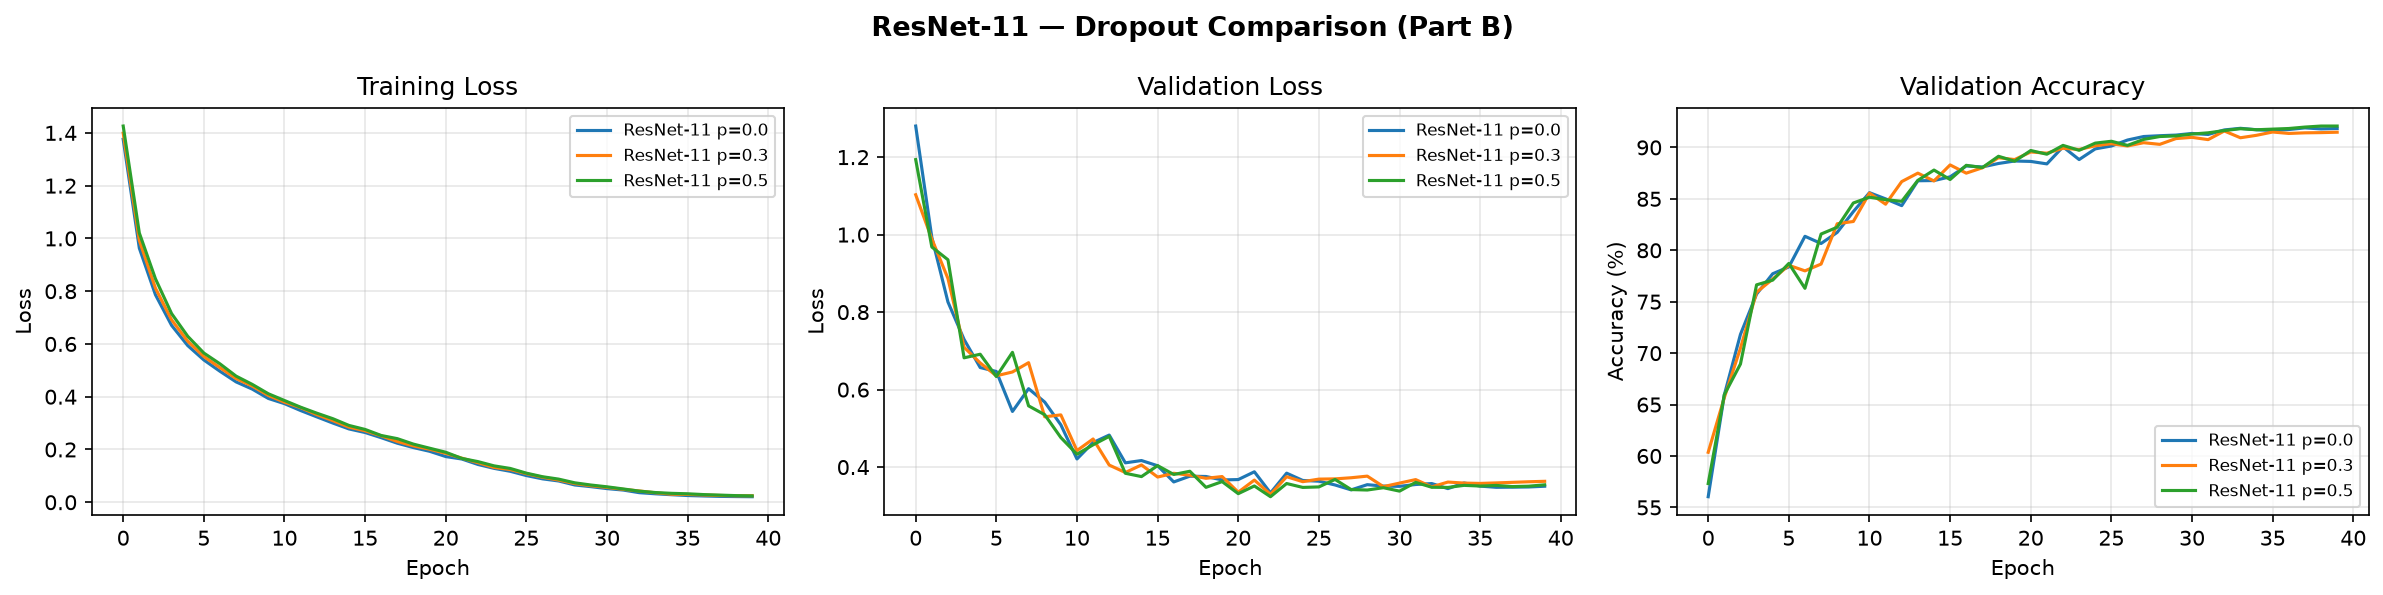
\includegraphics[width=\linewidth]{../../hw1/output/q3/3b_r11_dropout.png}
            \caption{Drouput = 0.3}
            \label{fig:3b_r11}
        \end{subfigure}
        \hfill
        \begin{subfigure}{\linewidth}
            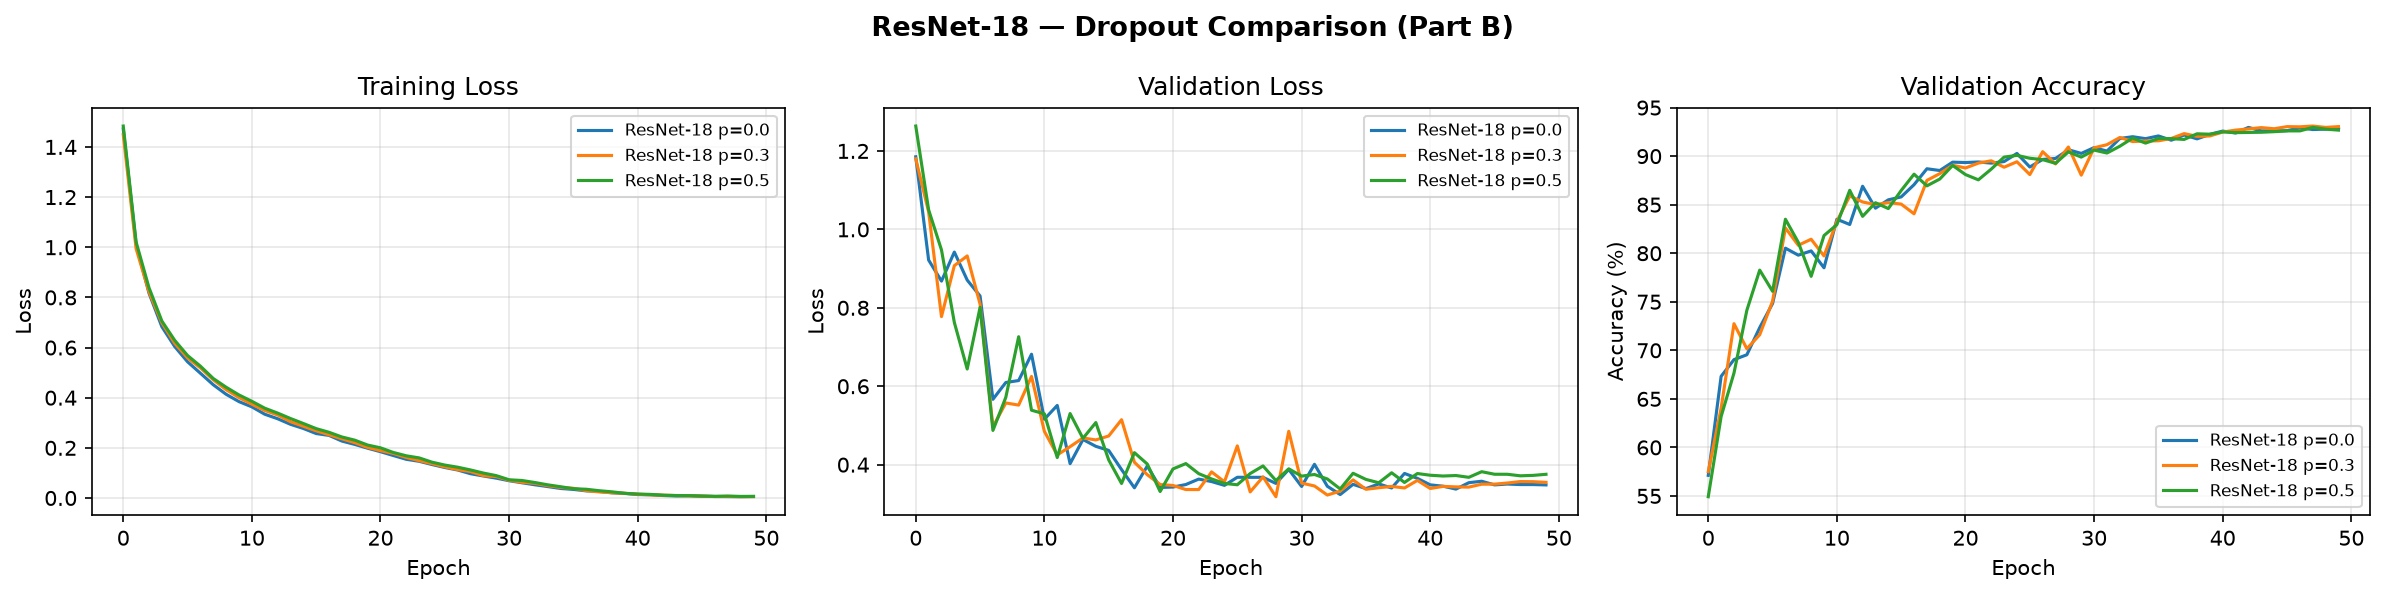
\includegraphics[width=\linewidth]{../../hw1/output/q3/3b_r18_dropout.png}
            \caption{Drouput = 0.5}
            \label{fig:3b_r18}
        \end{subfigure}
        \caption{Training Curves for Different Dropouts of ResNet Models}
    \end{center}
\end{figure}

\begin{figure}[H]
    \begin{center}
            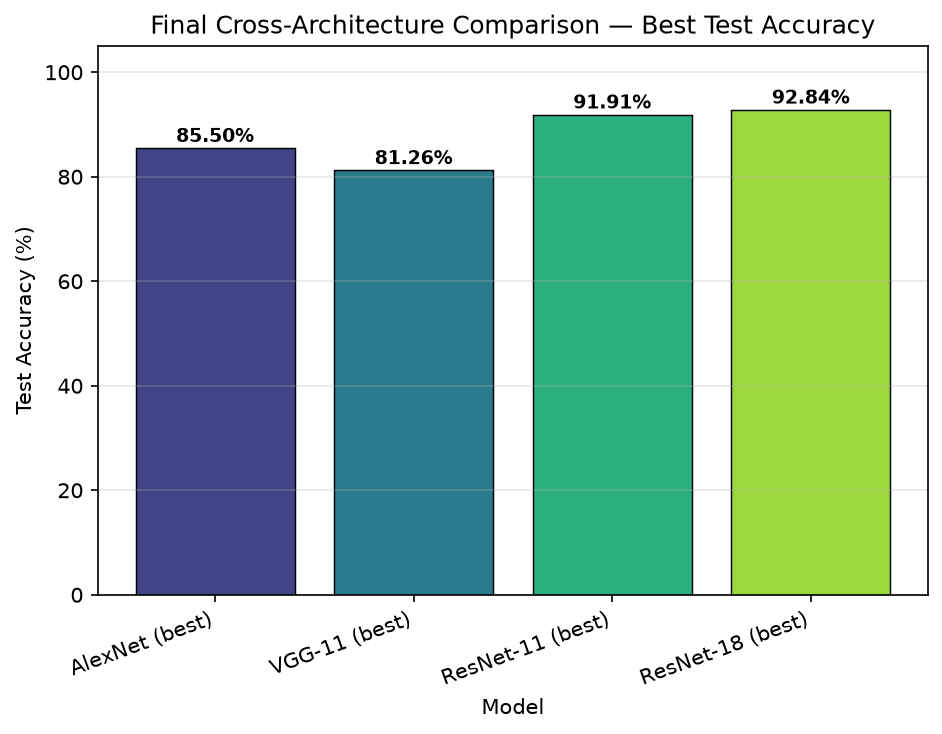
\includegraphics[width=\linewidth]{../../hw1/output/q3/3b_final_comparison.png}
            \caption{\textbf{Comparison between Cross-Model Dropouts}}
            \label{fig:3b_modelDropComp}
    \end{center}
\end{figure}

As discussed before, depth adds to the accuracy of the model training but the resolution of the input and the requirements also need to be taken into consideration. At the low resolution of CIFAR-10's images across such broad categories, the high depth of ResNet-18 was not required. In addition, as we move across families the architecture of each scale faster than the performance outputs that we have witnessed. In addition, the time needed to train each model should be taken into consideration. The modified AlexNet, had a reasonable baseline accuracy of 85.5\% while take around 3.5 seconds per epoch. ResNet-11 on the other hand had a standard epoch training time of 13.5 seconds for a baseline accuracy of 91.82. That means for an additional 10 seconds per epoch we only got an increase of 1.6\%. This is a sharp decline in performance over complexity of the model and the time take to train the model. Therefore, picking a suitable architecture with clear constraints is the best solution. In this case, I would suggest using the modified AlexNet.

\end{document}